% Template KLTN cho SV trường ĐHKHTN
% Liên hệ: nqminh@fit.hcmus.edu.vn
% Last update: 30/11/2016

% Chú ý: đọc các phần chú ý đóng khung của file này và chỉnh lại cho phù hợp.
% Trước khi build, xóa hết các file được tạo ra trong quá trình build trước đó (tất cả các file nằm ở thư mục gốc, trừ file main.tex này), và build theo thứ tự: BIB > PDF > PDF.
% Nếu cập nhật tài liệu tham khảo, cũng cần build lại theo cách trên.

% Đã kiểm tra trên MikTeX 2.9 Windows, TexMaker, Winshell

\documentclass[oneside,a4paper,12pt]{extreport}

% Font tiếng Việt
\usepackage[T5]{fontenc}
\usepackage[utf8]{inputenc}
\usepackage{times} % Times New Roman
\usepackage{pgfplots}
\usepgfplotslibrary{groupplots}
\usepackage{enumitem}     
\DeclareTextSymbolDefault{\DH}{T1}

\usepackage{titlesec}
\setcounter{secnumdepth}{3}
\titleformat{\paragraph}
{\normalfont\normalsize\bfseries}{\theparagraph}{1em}{}
\titlespacing*{\paragraph}
{0pt}{3.25ex plus 1ex minus .2ex}{1.5ex plus .2ex}

% Tài liệu tham khảo
\usepackage[
	sorting=nty,
	backend=biber,
	defernumbers=true]{biblatex}
\usepackage[unicode]{hyperref} % Bookmark tiếng Việt
\addbibresource{Ref/ref.bib}

\makeatletter
\def\blx@maxline{77}
\makeatother

% Chèn hình, các hình trong luận văn được để trong thư mục Images/
\usepackage{graphicx}
\graphicspath{ {Images/} }

% Chèn và định dạng mã nguồn
\usepackage{listings}
\usepackage{color}
\definecolor{codegreen}{rgb}{0,0.6,0}
\definecolor{codegray}{rgb}{0.5,0.5,0.5}
\definecolor{codepurple}{rgb}{0.58,0,0.82}
\definecolor{backcolour}{rgb}{0.95,0.95,0.92}
\lstdefinestyle{mystyle}{
    backgroundcolor=\color{backcolour},   
    commentstyle=\color{codegreen},
    keywordstyle=\color{magenta},
    numberstyle=\tiny\color{codegray},
    stringstyle=\color{codepurple},
    basicstyle=\footnotesize,
    breakatwhitespace=false,         
    breaklines=true,                 
    captionpos=b,                    
    keepspaces=true,                 
    numbers=left,                    
    numbersep=5pt,                  
    showspaces=false,                
    showstringspaces=false,
    showtabs=false,                  
    tabsize=2
}
\lstset{style=mystyle}

% Chèn và định dạng mã giả
\usepackage{amsmath}
\usepackage{algorithm}
\usepackage[noend]{algpseudocode}
\makeatletter
\def\BState{\State\hskip-\ALG@thistlm}
\makeatother

% Bảng biểu
\usepackage{multirow}
\usepackage{array}
\usepackage{booktabs}
\newcolumntype{L}[1]{>{\raggedright\let\newline\\\arraybackslash\hspace{0pt}}m{#1}}
\newcolumntype{C}[1]{>{\centering\let\newline\\\arraybackslash\hspace{0pt}}m{#1}}
\newcolumntype{R}[1]{>{\raggedleft\let\newline\\\arraybackslash\hspace{0pt}}m{#1}}

% Đổi tên mặc định
%\renewcommand{\chaptername}{Chương}
%\renewcommand{\figurename}{Hình}
%\renewcommand{\tablename}{Bảng}
%\renewcommand{\contentsname}{Mục lục}
%\renewcommand{\listfigurename}{Danh sách hình}
%\renewcommand{\listtablename}{Danh sách bảng}
%\renewcommand{\appendixname}{Phụ lục}

% Dãn dòng 1.5
\usepackage{setspace}
\onehalfspacing

% Thụt vào đầu dòng
\usepackage{indentfirst}

% Canh lề
\usepackage[
  top=35mm,
  bottom=30mm,
  left=35mm,
  right=20mm,
  includefoot]{geometry}
  
% Trang bìa
\usepackage{tikz}
\usetikzlibrary{calc}
\newcommand\HRule{\rule{\textwidth}{1pt}}


% ========================================================================================= %
% CHÚ Ý: Thông tin chung về KLTN - sinh viên điền vào đây để tự động update các trang khác  %
% ========================================================================================= %
\newcommand{\tenSV}{Thai~Thien} % Dấu ~ là khoảng trắng không được tách (các chữ nối với nhau bằng dấu ~ sẽ nằm cùng 1 dòng
\newcommand{\mssv}{1351040}
\newcommand{\tenSVt}{Van~Duy~Vinh} % Dấu ~ là khoảng trắng không được tách (các chữ nối với nhau bằng dấu ~ sẽ nằm cùng 1 dòng
\newcommand{\mssvt}{1351050}
\newcommand{\tenKL}{Deep~learning for Sentiment~Analysis of Movie~Reviews} % Chú ý dấu ~ trong tên khóa luận
\newcommand{\tenGVHD}{Nghiêm~Quốc~Minh}
\newcommand{\tenBM}{Công nghệ tri thức}

\newcommand{\floor}[1]{\lfloor #1 \rfloor}
\newcommand{\norm}[1]{\left\lVert #1 \right\rVert}

\usepackage{bm}
\usepackage{float}
\floatstyle{plain}
\restylefloat{table}
\usepackage{amsfonts}

\usepackage{blindtext}



\begin{document}

\begin{titlepage}

\begin{center}
UNIVERSITY OF SCIENCE\\
ADVANCED PROGRAM IN COMPUTER SCIENCE\\[2cm]
%BỘ MÔN \MakeUppercase{\tenBM}\\[2cm]

{ \Large \bfseries \MakeUppercase{\tenSV ~-~ \mssv} \\[2cm]
\Large \bfseries \MakeUppercase{\tenSVt ~-~ \mssvt} } %Nếu có 2 sinh viên thì chèn thêm 1 dòng vào đây, đồng thời chú ý canh trang cho phù hợp

{ \LARGE \bfseries \MakeUppercase{\tenKL} \\[2cm] } %SV có thể tự điền tên vào nếu cần xuống dòng chỗ phù hợp

\Large BACHELOR OF SCIENCE IN COMPUTER SCIENCE\\[2cm]

%\Large GIÁO VIÊN HƯỚNG DẪN\\
%\MakeUppercase{\tenGVHD} \\[2cm]

\begin{tikzpicture}[remember picture, overlay]
  \draw[line width = 2pt] ($(current page.north west) + (2cm,-2cm)$) rectangle ($(current page.south east) + (-1.5cm,2cm)$);
\end{tikzpicture}

\vfill
HO CHI MINH CITY, \the\year

\end{center}

\end{titlepage}


\begin{titlepage}

\begin{center}
UNIVERSITY OF SCIENCE\\
ADVANCED PROGRAM IN COMPUTER SCIENCE\\[2cm]
%BỘ MÔN \MakeUppercase{\tenBM}\\[2cm]

{ \Large \bfseries \MakeUppercase{\tenSV ~-~ \mssv} \\
\Large \bfseries \MakeUppercase{\tenSVt ~-~ \mssvt} \\[2cm] } %Nếu có 2 sinh viên thì chèn thêm 1 dòng vào đây, đồng thời chú ý canh trang cho phù hợp
 
{ \LARGE \bfseries \MakeUppercase{\tenKL} \\[2cm] } %SV có thể tự điền tên vào nếu cần xuống dòng chỗ phù hợp

\Large BACHELOR OF SCIENCE IN COMPUTER SCIENCE\\[2cm]

\Large THESIS ADVISOR\\
\MakeUppercase{\tenGVHD} \\[2cm]

\begin{tikzpicture}[remember picture, overlay]
  \draw[line width = 2pt] ($(current page.north west) + (2cm,-2cm)$) rectangle ($(current page.south east) + (-1.5cm,2cm)$);
\end{tikzpicture}

\vfill
HO CHI MINH CITY, \the\year

\end{center}

\end{titlepage}

% Sasu trang Title, các bạn chèn nhận xét gủa GVHD và GVPB. Nhận xét sẽ được giáo vụ phát sau buổi bảo vệ để các bạn đóng quyển.

\pagenumbering{roman} % Đánh số i, ii, iii, ...

%\addcontentsline{toc}{chapter}{Lời cam đoan}
%\chapter*{Lời cam đoan}
\label{reassurances}

Tôi xin cam đoan đây là công trình nghiên cứu của riêng tôi. Các số liệu và kết quả nghiên cứu trong luận văn này là trung thực và không trùng lặp với các đề tài khác.

\addcontentsline{toc}{chapter}{ACKNOWLEDGMENTS}
\chapter*{ACKNOWLEDGMENTS}
\label{thanks}

Tôi xin chân thành cảm ơn~\ldots

Xin cám ơn!

\vspace{3cm}
\hspace{7cm}
\begin{minipage}[ht]{0.48\textwidth}
\begin{center}
Tp. Hồ Chí Minh, ngày ... tháng ... năm 2016

Sinh viên thực hiện

\tenSV  ~~~~~~~   \tenSVt 
\end{center}
\end{minipage}


%\addcontentsline{toc}{chapter}{Đề cương chi tiết}
%\begin{flushleft}
Khoa Công Nghệ Thông Tin\\
Bộ môn \tenBM\\[2cm]
\end{flushleft}

\begin{center}
\LARGE \textbf{ĐỀ CƯƠNG CHI TIẾT}
\end{center}

\begin{tabular}{|L{15cm}|}
\hline
\textbf{Tên đề tài:} \tenKL \\
\hline
\textbf{Giáo viên hướng dẫn:} \tenGVHD \\
\hline
\textbf{Thời gian thực hiện:} 01/01/2000-01/01/2001\\
\hline
\textbf{Sinh viên thực hiện:}
 \tenSV ~-~ \mssv \\
 \tenSVt ~-~ \mssvt \\
\hline
\textbf{Loại đề tài:} Tìm hiểu công nghệ (có hoặc không ứng dụng minh hoạ), Xây dựng ứng dụng, ...\\
\hline
\end{tabular}\\[1cm]

\begin{tabular}{|L{15cm}|}
\hline
\textbf{Nội dung đề tài:} mô tả chi tiết nội dung đề tài, yêu cầu, phương pháp thực hiện, kết quả đạt được, ...\\
\hline
\textbf{Kế hoạch thực hiện:} mô tả chi tiết thời gian của các giai đoạn thực hiện và phân công công việc của từng thành viên trong nhóm\\
\hline
\end{tabular}\\[1cm]

\begin{tabular}{C{8cm}C{8cm}}
Xác nhận của GVHD & Ngày ... tháng ... năm 2016 \\
    ~\\~          & ~\\~                        \\
\tenGVHD          & \tenSV  ~~~~~~~~~~~~~~~~ \tenSVt
\end{tabular}


% Mục lục, danh sách hình, danh sách bảng
\addcontentsline{toc}{chapter}{TABLE OF CONTENTS}
\tableofcontents
\listoffigures
\listoftables

\addcontentsline{toc}{chapter}{ABSTRACT}
\chapter*{ABSTRACT}
\label{tomtat}

A large proportion of our perceptions of the world around us is made up of opinions.
In large scale, opinions run our economy, shape our government and drive our history.
The ability to comprehend and control opinions brings great power.
Since the last decade, opinions have been expressed in the highest speed, volume, and complexity ever recorded in history.
As a result, the task of tracking the flow of opinions on the Internet become impossible without automation.
To fill the niche, Sentiment Analysis is the field of study that investigates the computational method for analyzing opinions.
In this field, one significant problem is to classify the sentiment expressed by a sentence.
This problem is named Sentence-level Sentiment Analysis.

The purpose of this thesis is to increase the classification accuracy on the task of sentence-level Sentiment Analysis.
For this purpose, three approaches were explored.
In the first approach, we tried to improve Recursive Neural Networks by parameterizing their composition functions with respect to local syntactic information at each node in the parse tree.
For our second approach, we recognized that one major obstacle of this task is the lack of context and knowledge in the small training set.
To tackle this problem, we utilized Glove method to do Transfer Learning on a large amount of document-level labeled sentiment data.
In the third approach, we combined Convolution Neural Networks with Recursive Neural Networks, which result in new sophisticated networks architect.
To mitigate the risk posed by training large networks on small training dataset, we experimented with several unsupervised pre-training methods which also types of Transfer Learning.

We evaluated our models on the public Stanford Sentiment Treebank dataset with binary setting.
We were able to outperform the state-of-the-art model by a good margin in terms average accuracy of 5 runs.


\clearpage

\pagenumbering{arabic} % Đánh số 1, 2, 3, ...
% intro 15
% related work 10
% method 15
% result and discuss 10
% conclusion  5
% => 55 
% Các chương nội dung
\chapter{Introduction}
\section{Context and purpose of this thesis}

\section{Contributions of this thesis}

\section{Structure of this thesis}


\chapter{Background}

\section{Sentiment Analysis}
In the nutshell, sentiment analysis is to determine whether the opinion about a specific product, event, organization is positive or negative.  
\subsection{The need for sentiment analysis}
Every business need feedback from customer. Feedback help company know their product strength and weakness, drive business strategy. For example, fix the flaw in product, target new customer segment or halt a campaign. Traditional, company would survey their customer to collect feedback.  The feedback collected from direct survey are limited for many reason, such as low population. 

With the growth of social network and e-commerce, more and more people post their opinion online via blog, social network (Facebook, Twitter), e-commerce site (Amazon, eBay). Company want to take advantage of these data. Thus, a automate system to analysis opinion are in demand. 
            
\subsection{The challenges}
Lorem ipsum dolor sit amet, consectetur adipiscing elit, sed do eiusmod tempor incididunt ut labore et dolore magna aliqua. Ut enim ad minim veniam, quis nostrud exercitation ullamco laboris nisi ut aliquip ex ea commodo consequat. Duis aute irure dolor in reprehenderit in voluptate velit esse cillum dolore eu fugiat nulla pariatur. Excepteur sint occaecat cupidatat non proident, sunt in culpa qui officia deserunt mollit anim id est laborum.

\subsection{Different levels in sentiment analysis}
\subsubsection{Document-level}
Document-level sentiment analysis is to determine whether a document (usually a full review) about a specific entity (a product, location, service, ...) is positive or negative. For example, \cite{pang2002thumbs} perform document-level sentiment analysis on movies review data.
\subsubsection{Sentence-level}
Sentence-level sentiment analysis is to determine whether a sentence expressed positive, negative. In this thesis, we focus our study on sentence-level sentiment analysis \cite{liu2012sentiment}. 
\subsubsection{Aspect-level}
Aspect-level  sentiment analysis purpose is to determine opinion, whether positive or negative, against specific aspect of entity \cite{liu2012sentiment}. 

\section{Feedforward neural network}
Feedforward neural network is a network whether unit in the graph does not form a cycle \cite{Goodfelloetal2016}. 

Each feedforward neural network consist at least one input layer, one output layer. Each layer contain one or more neurons (network nodes). Each neuron consist of a linear activation or non-linear activation function. 

Each node have an activation function. There are two type of activation function: Linear and non-linear. 

Example of linear function: \\
\[f(x) = Wx + b \]

Example of non-linear function: \\
\[f(x) = tanh(x) \]
\[f(x) =\frac{1}{1+e^{-x}} \]

\subsection{Single-layer perceptron}
Singlelayer perceptron is a feedforward neural network only have one input layer and one output layer of neuron unit (See fig \ref{fig:singleperceptron}). Singlelayer perceptron cannot solve some problem such as XOR.
\begin{figure}[H]
	\centering
	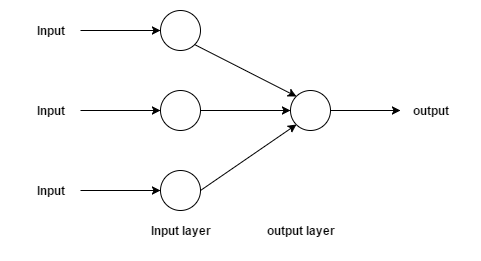
\includegraphics[width=0.7\linewidth]{../figure/singleperceptron}
	\caption[Single-layer Perceptron]{Single-layer Perceptron}
	\label{fig:singleperceptron}
\end{figure}



\subsection{Multi-layer perceptron}
Multilayer perceptron (MLP) is a feedforward neural network consist of 2 or more layer (See fig \ref{fig:multilayerperceptron}). First layer called input layer. Last layer called output layer. All layer between input and output layer are hidden layer. A series of linear function is equal to 2 layer perceptron. Hence, MLP always contain non-linear activation function. In MLP, every unit of previous layer connect to all unit in next layer.

\begin{figure}[H]
	\centering
	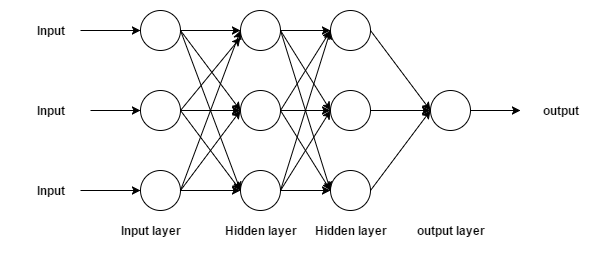
\includegraphics[width=0.7\linewidth]{../figure/multilayerperceptron}
	\caption[Multi-layer Perceptron]{Multi-layer Perceptron}
	\label{fig:multilayerperceptron}
\end{figure}

\subsection{Forward pass}
Forward pass, or forward propagation, is a process which information from input x flow through the network to output y. In MLP forward pass, an input x is feed through first layer, also known as input layer. Output from first layer is use as input for second layer, and so on until it reach last layer, output layer. Output from output layer are output of MLP. 

For example: a MLP with 4 activation function: $f(x)$, $g(x)$, $h(x)$, $k(x)$. With $f(x)$ is input layer, $k(x)$ is output layer, and $g(x), h(x)$ are hidden layers .With input $x$, then MLP has output $ y = k(h(g(f(x))))$.

\subsection{Cost function}
Cost function $J(\theta)$  is a measurement how far predicted  $\hat y$ from expected label $y$. When our model predict exactly the labeled output, then cost function is zero. The problem is to minimize the cost function. Cost function of MLP dependent on output layer.

For most of our experiment, we would use softmax output layer and cross-entropy loss function.
\subsection{Backward pass}





\section{Convolution Neural Network}
Lorem ipsum dolor sit amet, consectetur adipiscing elit, sed do eiusmod tempor incididunt ut labore et dolore magna aliqua. Ut enim ad minim veniam, quis nostrud exercitation ullamco laboris nisi ut aliquip ex ea commodo consequat. Duis aute irure dolor in reprehenderit in voluptate velit esse cillum dolore eu fugiat nulla pariatur. Excepteur sint occaecat cupidatat non proident, sunt in culpa qui officia deserunt mollit anim id est laborum.
\subsection{Architect}
Lorem ipsum dolor sit amet, consectetur adipiscing elit, sed do eiusmod tempor incididunt ut labore et dolore magna aliqua. Ut enim ad minim veniam, quis nostrud exercitation ullamco laboris nisi ut aliquip ex ea commodo consequat. Duis aute irure dolor in reprehenderit in voluptate velit esse cillum dolore eu fugiat nulla pariatur. Excepteur sint occaecat cupidatat non proident, sunt in culpa qui officia deserunt mollit anim id est laborum.
\subsection{Back propagation}
Lorem ipsum dolor sit amet, consectetur adipiscing elit, sed do eiusmod tempor incididunt ut labore et dolore magna aliqua. Ut enim ad minim veniam, quis nostrud exercitation ullamco laboris nisi ut aliquip ex ea commodo consequat. Duis aute irure dolor in reprehenderit in voluptate velit esse cillum dolore eu fugiat nulla pariatur. Excepteur sint occaecat cupidatat non proident, sunt in culpa qui officia deserunt mollit anim id est laborum.
\section{Recurrent Neural Network}
Lorem ipsum dolor sit amet, consectetur adipiscing elit, sed do eiusmod tempor incididunt ut labore et dolore magna aliqua. Ut enim ad minim veniam, quis nostrud exercitation ullamco laboris nisi ut aliquip ex ea commodo consequat. Duis aute irure dolor in reprehenderit in voluptate velit esse cillum dolore eu fugiat nulla pariatur. Excepteur sint occaecat cupidatat non proident, sunt in culpa qui officia deserunt mollit anim id est laborum.
\subsection{RNN}
Lorem ipsum dolor sit amet, consectetur adipiscing elit, sed do eiusmod tempor incididunt ut labore et dolore magna aliqua. Ut enim ad minim veniam, quis nostrud exercitation ullamco laboris nisi ut aliquip ex ea commodo consequat. Duis aute irure dolor in reprehenderit in voluptate velit esse cillum dolore eu fugiat nulla pariatur. Excepteur sint occaecat cupidatat non proident, sunt in culpa qui officia deserunt mollit anim id est laborum.
\subsection{LSTM}
Lorem ipsum dolor sit amet, consectetur adipiscing elit, sed do eiusmod tempor incididunt ut labore et dolore magna aliqua. Ut enim ad minim veniam, quis nostrud exercitation ullamco laboris nisi ut aliquip ex ea commodo consequat. Duis aute irure dolor in reprehenderit in voluptate velit esse cillum dolore eu fugiat nulla pariatur. Excepteur sint occaecat cupidatat non proident, sunt in culpa qui officia deserunt mollit anim id est laborum.
\subsection{Back propagation}
Lorem ipsum dolor sit amet, consectetur adipiscing elit, sed do eiusmod tempor incididunt ut labore et dolore magna aliqua. Ut enim ad minim veniam, quis nostrud exercitation ullamco laboris nisi ut aliquip ex ea commodo consequat. Duis aute irure dolor in reprehenderit in voluptate velit esse cillum dolore eu fugiat nulla pariatur. Excepteur sint occaecat cupidatat non proident, sunt in culpa qui officia deserunt mollit anim id est laborum.
\section{Distributed Representations of Words}
\subsection{Definition}
Lorem ipsum dolor sit amet, consectetur adipiscing elit, sed do eiusmod tempor incididunt ut labore et dolore magna aliqua. Ut enim ad minim veniam, quis nostrud exercitation ullamco laboris nisi ut aliquip ex ea commodo consequat. Duis aute irure dolor in reprehenderit in voluptate velit esse cillum dolore eu fugiat nulla pariatur. Excepteur sint occaecat cupidatat non proident, sunt in culpa qui officia deserunt mollit anim id est laborum.
\subsection{work2vec}
Lorem ipsum dolor sit amet, consectetur adipiscing elit, sed do eiusmod tempor incididunt ut labore et dolore magna aliqua. Ut enim ad minim veniam, quis nostrud exercitation ullamco laboris nisi ut aliquip ex ea commodo consequat. Duis aute irure dolor in reprehenderit in voluptate velit esse cillum dolore eu fugiat nulla pariatur. Excepteur sint occaecat cupidatat non proident, sunt in culpa qui officia deserunt mollit anim id est laborum.
\subsection{Glove}
Lorem ipsum dolor sit amet, consectetur adipiscing elit, sed do eiusmod tempor incididunt ut labore et dolore magna aliqua. Ut enim ad minim veniam, quis nostrud exercitation ullamco laboris nisi ut aliquip ex ea commodo consequat. Duis aute irure dolor in reprehenderit in voluptate velit esse cillum dolore eu fugiat nulla pariatur. Excepteur sint occaecat cupidatat non proident, sunt in culpa qui officia deserunt mollit anim id est laborum.
\subsection{Different methods to produce word embedding}
Lorem ipsum dolor sit amet, consectetur adipiscing elit, sed do eiusmod tempor incididunt ut labore et dolore magna aliqua. Ut enim ad minim veniam, quis nostrud exercitation ullamco laboris nisi ut aliquip ex ea commodo consequat. Duis aute irure dolor in reprehenderit in voluptate velit esse cillum dolore eu fugiat nulla pariatur. Excepteur sint occaecat cupidatat non proident, sunt in culpa qui officia deserunt mollit anim id est laborum.
\section{Parse tree in NLP}
Lorem ipsum dolor sit amet, consectetur adipiscing elit, sed do eiusmod tempor incididunt ut labore et dolore magna aliqua. Ut enim ad minim veniam, quis nostrud exercitation ullamco laboris nisi ut aliquip ex ea commodo consequat. Duis aute irure dolor in reprehenderit in voluptate velit esse cillum dolore eu fugiat nulla pariatur. Excepteur sint occaecat cupidatat non proident, sunt in culpa qui officia deserunt mollit anim id est laborum.
\subsection{Constituency Parse Tree}
Lorem ipsum dolor sit amet, consectetur adipiscing elit, sed do eiusmod tempor incididunt ut labore et dolore magna aliqua. Ut enim ad minim veniam, quis nostrud exercitation ullamco laboris nisi ut aliquip ex ea commodo consequat. Duis aute irure dolor in reprehenderit in voluptate velit esse cillum dolore eu fugiat nulla pariatur. Excepteur sint occaecat cupidatat non proident, sunt in culpa qui officia deserunt mollit anim id est laborum.
\subsection{Dependency Parse Tree}
Lorem ipsum dolor sit amet, consectetur adipiscing elit, sed do eiusmod tempor incididunt ut labore et dolore magna aliqua. Ut enim ad minim veniam, quis nostrud exercitation ullamco laboris nisi ut aliquip ex ea commodo consequat. Duis aute irure dolor in reprehenderit in voluptate velit esse cillum dolore eu fugiat nulla pariatur. Excepteur sint occaecat cupidatat non proident, sunt in culpa qui officia deserunt mollit anim id est laborum.
\section{Recursive Neural Network}
Lorem ipsum dolor sit amet, consectetur adipiscing elit, sed do eiusmod tempor incididunt ut labore et dolore magna aliqua. Ut enim ad minim veniam, quis nostrud exercitation ullamco laboris nisi ut aliquip ex ea commodo consequat. Duis aute irure dolor in reprehenderit in voluptate velit esse cillum dolore eu fugiat nulla pariatur. Excepteur sint occaecat cupidatat non proident, sunt in culpa qui officia deserunt mollit anim id est laborum.
\subsection{RNN: Recursive Neural Network}
Lorem ipsum dolor sit amet, consectetur adipiscing elit, sed do eiusmod tempor incididunt ut labore et dolore magna aliqua. Ut enim ad minim veniam, quis nostrud exercitation ullamco laboris nisi ut aliquip ex ea commodo consequat. Duis aute irure dolor in reprehenderit in voluptate velit esse cillum dolore eu fugiat nulla pariatur. Excepteur sint occaecat cupidatat non proident, sunt in culpa qui officia deserunt mollit anim id est laborum.
\subsection{MV-RNN: Matrix-Vector RNN}
Lorem ipsum dolor sit amet, consectetur adipiscing elit, sed do eiusmod tempor incididunt ut labore et dolore magna aliqua. Ut enim ad minim veniam, quis nostrud exercitation ullamco laboris nisi ut aliquip ex ea commodo consequat. Duis aute irure dolor in reprehenderit in voluptate velit esse cillum dolore eu fugiat nulla pariatur. Excepteur sint occaecat cupidatat non proident, sunt in culpa qui officia deserunt mollit anim id est laborum.
\subsection{RNTN:Recursive Neural Tensor}
Lorem ipsum dolor sit amet, consectetur adipiscing elit, sed do eiusmod tempor incididunt ut labore et dolore magna aliqua. Ut enim ad minim veniam, quis nostrud exercitation ullamco laboris nisi ut aliquip ex ea commodo consequat. Duis aute irure dolor in reprehenderit in voluptate velit esse cillum dolore eu fugiat nulla pariatur. Excepteur sint occaecat cupidatat non proident, sunt in culpa qui officia deserunt mollit anim id est laborum. Network
\section{Programming Framework}
\subsubsection{RNTN:Recursive Neural Tensor}
Lorem ipsum dolor sit amet, consectetur adipiscing elit, sed do eiusmod tempor incididunt ut labore et dolore magna aliqua. Ut enim ad minim veniam, quis nostrud exercitation ullamco laboris nisi ut aliquip ex ea commodo consequat. Duis aute irure dolor in reprehenderit in voluptate velit esse cillum dolore eu fugiat nulla pariatur. Excepteur sint occaecat cupidatat non proident, sunt in culpa qui officia deserunt mollit anim id est laborum. Network
\subsection{Torch}
Torch \footnote{http://torch.ch/} is Lua scientific computing framework. Torch support high performing matrix calculation via multi-dimensional array call Tensor. Torch are built with C/C++, CUDA backend. Torch author choose Lua because Lua works well with C/C++ \cite{collobert2011torch7}.  Thus, Torch is high performing and support GPU. Torch have neural network package (nn) package. Computation graph must be define before forward pass. 
A simple, single linear layer network can be easily defined with few line of code (see listing \ref{lst:torchlinear}).

\begin{lstlisting}[caption={Simple linear layer in Torch},label={lst:torchlinear}, language={[5.1]Lua}]
-- simple y = Ax + b linear layer
l = nn.Linear(2,3)
-- forward pass
x = torch.Tensor(2)
y = l:forward(x) -- vector dimension of 3
\end{lstlisting}

However, when a model need multiple module, such as multilayer perceptron (MLP), these module must be put into container. Figure \ref{fig:nncontainer} illustrates on function of each nn container . In order to construct two-layer perception (eq \ref{eq:mlp}), linear, tanh and softmax module must be packed into sequential module (see listing \ref{lst:torchmlp}).

\begin{equation}
\label{eq:mlp}
\begin{aligned}
&h = tanh(W_1*x + b_1) \\
&y = softmax(W_2*h + b2)
\end{aligned}
\end{equation}


\begin{lstlisting}[caption={MLP in Torch},label={lst:torchmlp}, language={[5.1]Lua}]
model = nn.Sequential()
model:add(nn.Linear(2,3))
model:add(nn.Tanh())
model:add(nn.Linear(3,5))
model:add(nn.SoftMax())
-- forward
x = torch.Tensor(2)
y = model:forward(x)
\end{lstlisting}

Torch provide nngraph package support build more complicate model. For example, define MLP in (eq \ref{eq:mlp}) use nngraph (see listing \ref{lst:torchnngraph})

\begin{lstlisting}[caption={MLP using nngraph},label={lst:torchnngraph}, language={[5.1]Lua}]
model = nn.Sequential()
model:add(nn.Linear(2,3))
model:add(nn.Tanh())
model:add(nn.Linear(3,5))
model:add(nn.SoftMax())
-- forward
x = torch.Tensor(2)
y = model:forward(x)
\end{lstlisting}

Sample code on training a model, see Appendix \ref{lst:torchtrain}

\subsection{Theano}
Theano \footnote{\url{http://deeplearning.net/software/theano/}} is a deep learning library on Python. It basic function is similar to Torch: matrix calculation, support GPU. Theano is define-and-run schema, which a computer graph must be built before it is executed.

\begin{lstlisting}[caption={Define function in Theano},label={lst:theanof}, language={python}]
x = T.dmatrix('x')
y = T.dmatrix('y')
z = x + y
f = function([x, y], z)
f([[1, 1], [2, 2]], [[3, 3], [4, 4]])
# result [[4, 4], [6, 6]]
\end{lstlisting}

Comparing to Torch7, Theano are slower on most benchmark \cite{collobert2011torch7}. Theano does not provide nice template like linear layer. Thus, model must be defined from equation. It give researcher more control over mathematics aspect but cause more trouble for beginner. A sample code for MLP \ref{lst:theanomlp}. One more problem is that the 'define-and-run' scheme does not suitable for recursive neural network due to recompile the computation graph each training sample take time. 

\subsection{Pytorch}
PyTorch uses same backend as Torch. However, PyTorch specially designed for Python. Pytorch have pre-define module (Linear layer, Convolution layer) like Torch. However, Pytorch does not require to pack model into container. In Pytorch a network are defined in forward-pass thanks to Dynamic Neural Networks feature. Therefore, user can use Python control flow to define a network. For example, one can use for loop to run recurrent neural network (see listing \ref{lst:pytorchrnn}) .The features allows us to implement Recursive Neural Network for NLP, which the network change for every sample, much more easier. 

\begin{lstlisting}[caption={RNN},label={lst:pytorchrnn}, language={python}]
import torch
import torch.nn as nn
rnn = nn.RNNCell(10, 20)
seq_len = 10
input_dim = 100
hidden_dim = 150
input = Variable(torch.randn(seq_len, 1, input_dim))
hx = Variable(torch.zeros(1, hidden_dim))
output = []
for i in range(6):
    hx = rnn(input[i], hx)
    output.append(hx)
\end{lstlisting}

We also implement treelstm from original Torch7 \footnote{\url{https://github.com/stanfordnlp/treelstm}} sentiment classification task in PyTorch and publish on Github \footnote{\url{https://github.com/ttpro1995/TreeLSTMSentiment}}.   

We choose PyTorch because: 
\begin{itemize}
	\item Dynamic Neural Networks feature works well on data sequence with different length
	\item Intuitive framework
	\item Easy to install and run on CUDA
\end{itemize}





\hypertarget{chap:related}{\chapter{Related Works}}
\label{chap:related-work}
\section{Datasets}\label{sec:dataset}
\subsection{Stanford Sentiment Treebank} \label{sec:sst}
In this thesis, we used Standford Sentiment Treebank (SST) dataset\cite{socher2013recursive} for evaluating our models on task of sentence-level sentiment analysis. 
Original, the dataset was built based on Rotten Tomatoes Movie Review dataset\cite{Rotten-Tomato}\cite{socher2013recursive}. 
In total, Standford Sentiment Treebank contains 11,855 sentences. 
The dataset was split into training, validation and testing set which contains 8544, 1101 and 2210 sentences respectively (Fig.\ref{fig:sstfinegrain}).
Table \ref{table:sststatistic} shows the distribution of sentiment classes on training, validation and testing set. 

In this dataset, every sentences were parsed using Stanford (constituency) parser\cite{socher2013recursive}\footnote{Open source tool: \url{https://stanfordnlp.github.io/CoreNLP/}}, each phrase which is spanned by any sub-tree of the parse tree is then labeled with  a fined-grain sentiment label (see \textbf{Figure \ref{fig:sst}}). 
Fined-grain sentiment is a setting which partition all sentiments into 5 classes: "Positive", "Somewhat Positive", "Neutral", "Somewhat Nagative" and "Nagative"\cite{socher2013recursive} (a.k.a. \textbf{Fine-grained setting}).
There are total 215,154 phrases in the whole dataset. 

For \textbf{Binary setting}, there are only to sentiment classed on the whole dataset, which means all neutral sentiment sentences are removed, "Positive" and "Somewhat Positive" are merged into one class, the same rule applied on "Somewhat Negative" and "Negative"\cite{socher2013recursive}.   
After all "Neutral" sentences have been removed, there are 6920/872/1821 sentences remained in train/dev/test set (Fig. \ref{fig:sstbinary}).


Table \ref{table:sststatistic} show statistics by sentences of Sentiment Treebank Dataset.
SST dataset is publicly available online \footnote{https://nlp.stanford.edu/sentiment/index.html}. 

\begin{figure}[H]
    \begin{minipage}{\textwidth}
        \centering
        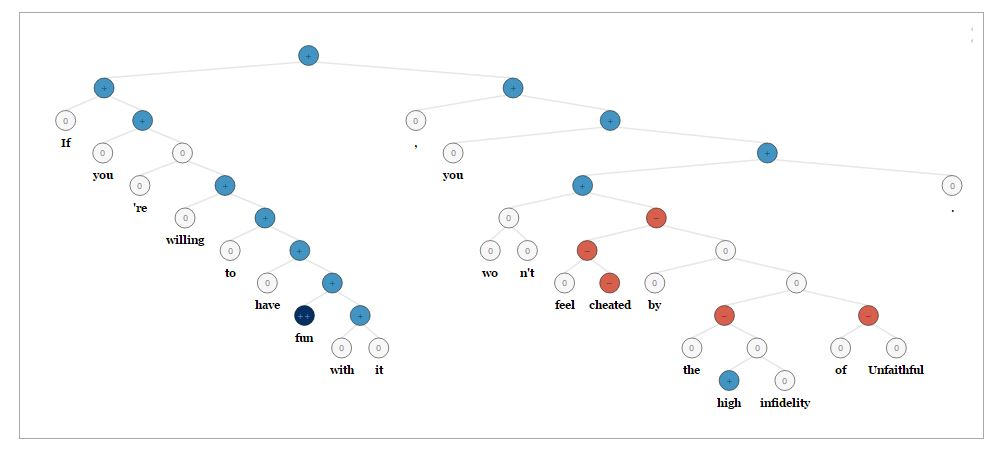
\includegraphics[width=0.9\linewidth]{figure/sst}
        \caption[A parsed sentence in SST]{A parsed sentence in SST \footnote{Render by Pytreebank \url{https://github.com/JonathanRaiman/pytreebank}}}
        \label{fig:sst}
    \end{minipage}
\end{figure}

\begin{figure}[H]
    \begin{minipage}{\textwidth}
        \centering
        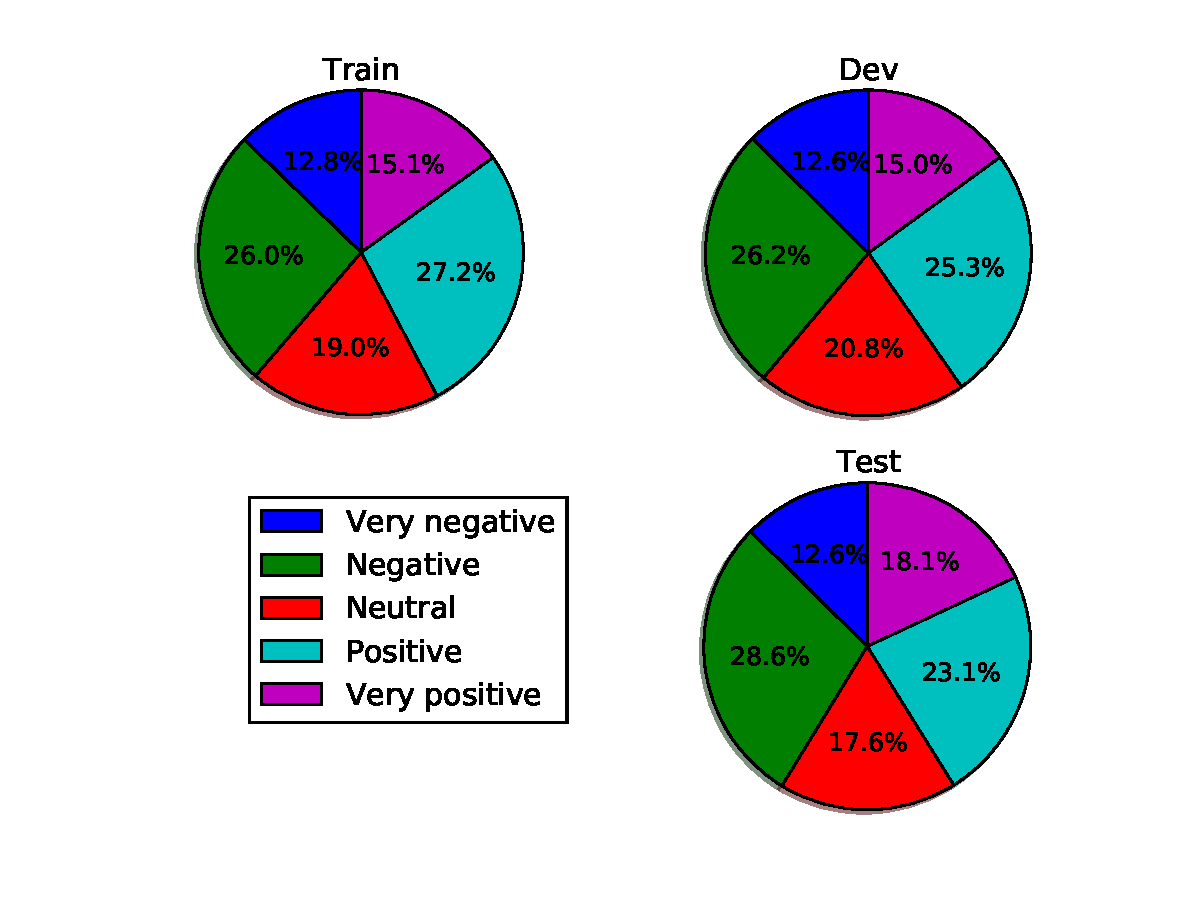
\includegraphics[width=0.9\linewidth]{figure/sstfinegrain}
        \caption[SST fine-grain sentiment distribution]{SST fine-grain sentiment distribution}
        \label{fig:sstfinegrain}
    \end{minipage}
\end{figure}

\begin{figure}[H]
    \begin{minipage}{\textwidth}
        \centering
        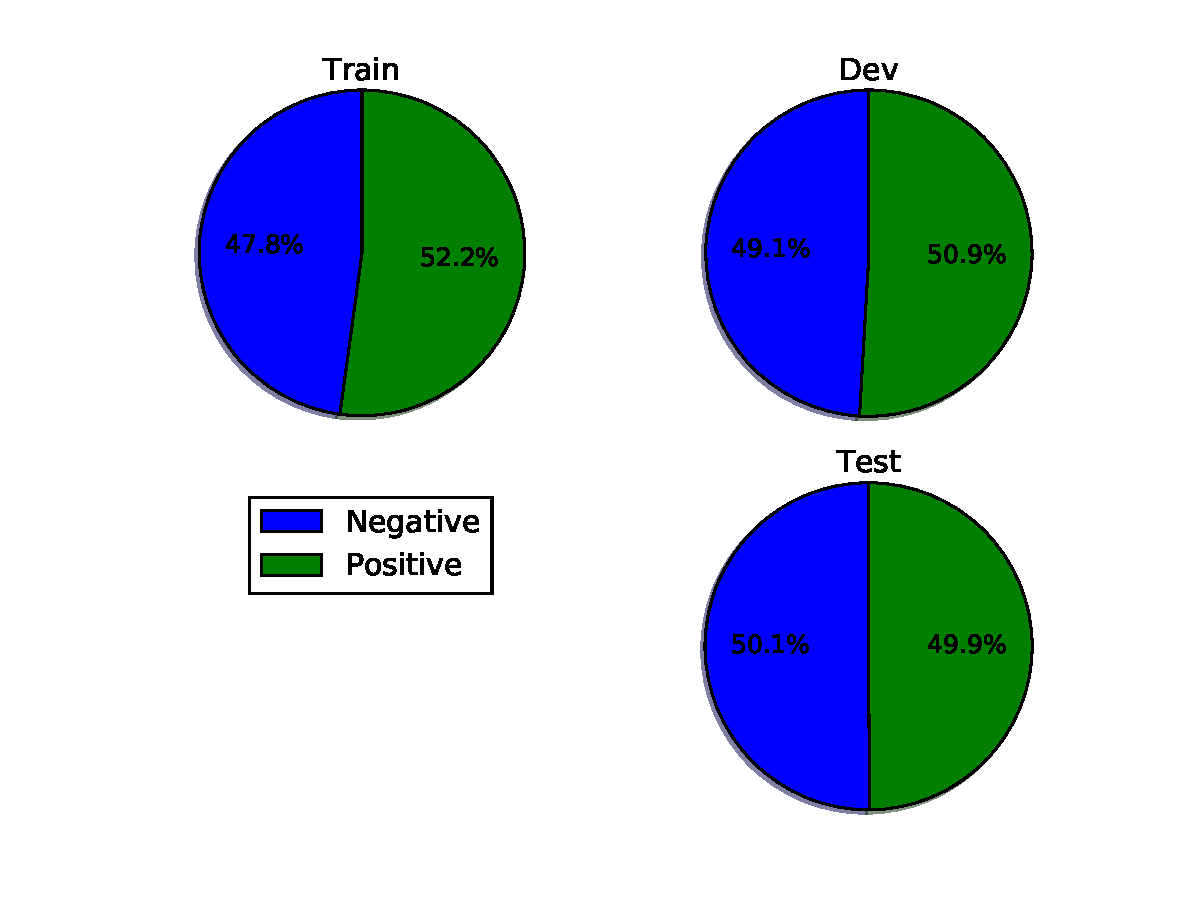
\includegraphics[width=0.9\linewidth]{figure/sstbinary}
        \caption[SST binary sentiment distribution]{SST binary sentiment distribution}
        \label{fig:sstbinary}
    \end{minipage}
\end{figure}

% Please add the following required packages to your document preamble:
% \usepackage{multirow}
\begin{table}[H]
    \centering
    \caption{SST statistics}
    \label{table:sststatistic}
    \begin{tabular}{lllll}
        Number of review       &               &      &                       &  \\ \cline{1-4}
        \multirow{5}{*}{Train} & Very Negative & 1092 & \multirow{2}{*}{3310} &  \\ \cline{2-3}
        & Negative      & 2218 &                       &  \\ \cline{2-4}
        & Neutral       & 1624 &                       &  \\ \cline{2-4}
        & Positive      & 2322 & \multirow{2}{*}{3610} &  \\ \cline{2-3}
        & Very positive & 1288 &                       &  \\ \cline{1-4}
        \multirow{5}{*}{Dev}   & Very Negative & 139  & \multirow{2}{*}{428}  &  \\ \cline{2-3}
        & Negative      & 289  &                       &  \\ \cline{2-4}
        & Neutral       & 229  &                       &  \\ \cline{2-4}
        & Positive      & 279  & \multirow{2}{*}{444}  &  \\ \cline{2-3}
        & Very positive & 165  &                       &  \\ \cline{1-4}
        \multirow{5}{*}{Test}  & Very Negative & 279  & \multirow{2}{*}{912}  &  \\ \cline{2-3}
        & Negative      & 633  &                       &  \\ \cline{2-4}
        & Neutral       & 389  &                       &  \\ \cline{2-4}
        & Positive      & 510  & \multirow{2}{*}{909}  &  \\ \cline{2-3}
        & Very Positive & 399  &                       &  \\ \cline{2-4}
    \end{tabular}
\end{table}

\subsection{Amazon Reviews dataset}\label{sec:amazon}
Amazon Reviews is a gigantic review dataset
which contains 142.8 million reviews from Amazon spanning May 1996 - July 2014\footnote{\url{http://jmcauley.ucsd.edu/data/amazon/}}.
Each review contains product review (rating, text, helpfulness vote) and metadata (descriptions, category information, price, brand, and image features)\cite{amazon-reviews}.
In this thesis, we only used a small part of Amazon Reviews.
These parts including Amazon Movies and TV reviews (7,850,072 reviews) \cite{mcauley2013hidden}, Amazon Book reviews (22,507,155 reviews) and the new Movies and TV reviews (4,607,047 reviews) \cite{McAuleyTSH15}\cite{HeM16}. 

Listing \ref{lst:amzreview} is a sample of book reviews. 
Amazon Book reviews and new Movies and TV dataset have the same format. Listing \ref{lst:oldamzreview} is a sample of Amazon Movies and TV reviews old dataset (7,850,072 reviews). 

\begin{lstlisting}[caption={Amazon reviews sample},label={lst:amzreview}]
    {
        "reviewerID": "AH2L9G3DQHHAJ",
        "asin": "0000000116",
        "reviewerName": "chris",
        "helpful": [5, 5],
        "reviewText": "Interesting Grisham tale of a lawyer that takes millions of dollars from his firm after faking his own death. Grisham usually is able to hook his readers early and ,in this case, doesn't play his hand to soon. The usually reliable Frank Mueller makes this story even an even better bet on Audiobook.",
        "overall": 4.0,
        "summary": "Show me the money!",
        "unixReviewTime": 1019865600,
        "reviewTime": "04 27, 2002"
    }
\end{lstlisting}

\begin{lstlisting}[caption={Old Amazon reviews sample},label={lst:oldamzreview}]
{
"reviewerID": "AH2L9G3DQHHAJ",
"asin": "0000000116",
"reviewerName": "chris",
"helpful": [5, 5],
"reviewText": "Interesting Grisham tale of a lawyer that takes millions of dollars from his firm after faking his own death. Grisham usually is able to hook his readers early and ,in this case, doesn't play his hand to soon. The usually reliable Frank Mueller makes this story even an even better bet on Audiobook.",
"overall": 4.0,
"summary": "Show me the money!",
"unixReviewTime": 1019865600,
"reviewTime": "04 27, 2002"
}
\end{lstlisting}

The differences between the old Amazon reviews dataset\footnote{\url{https://snap.stanford.edu/data/web-Amazon.html}} and new Amazon reviews dataset \footnote{\url{http://jmcauley.ucsd.edu/data/amazon/}} is that: 
They were gathered using different crawling methods, the author also solved the duplication problem in new the dataset\cite{amazon-reviews}.
Table \ref{table:moviereview} show number of reviews by overall.

\begin{table}[H]
    \centering
    \caption{New Movies and TV dataset}
    \label{table:moviereview}
    \begin{tabular}{@{}lllc@{}}
        \toprule
        & \multicolumn{3}{l}{Number of reviews}                         \\ \midrule
        5-Star & 2761408 & \multirow{2}{*}{3618913} & \multirow{5}{*}{4607047} \\ \cmidrule(r){1-2}
        4-Star & 857505  &                          &                          \\ \cmidrule(r){1-3}
        3-Star & \multicolumn{2}{l}{415369}         &                          \\ \cmidrule(r){1-3}
        2-Star & 233221  & \multirow{2}{*}{572765}  &                          \\ \cmidrule(r){1-2}
        1-Star & 339544  &                          &                          \\ \bottomrule
    \end{tabular}
\end{table}


\section{Neural network architects for sentence composition}\label{sec:composer}
\subsection{Recurrent neural networks}\label{sec:RNN}
In real life, we usually encounter a type of problems whose output (or output sequence) is determined by an variable-length sequence of input data points. 
Recurrent Neural Networks have been proven to be effective network architects when applying on this type of problems.  
Particularly in Natural Language Processing, various tasks enjoy dramatic improvements by using different variations of Recurrent Neural Networks, these tasks including:  speech recognition\cite{speech-lstm}\cite{MiaoGM15}, sentiment analysis\cite{treeLSTM}\cite{cnn-rnn}\cite{attention-gru}, text summarization\cite{RushCW15}\cite{NallapatiXZ16}, machine translation\cite{FiratCB16}\cite{SutskeverVL14}\cite{BritzGLL17}, language modeling\cite{mikolov-nlm}\cite{JozefowiczVSSW16} and more\cite{deep-nlp}\cite{Schmidhuber14}\cite{deeplearning-book}.

By definition, Recurrent Neural Networks are any Neural Networks which have at least a recurrent connection\cite{rnn-def} but we will describe several common types of Recurrent Neural Networks which closely related to this theses.

\subsubsection{Vanilla Recurrent Unit}\label{sec:vanilla-rnn}
Denoting input sequence as \(I = \{i_0,\ldots,i_n\}, \forall t, i_t \in \mathbb{R}^n\), Vanilla Recurrent unit can be expressed as the following recursive formula\cite{treeLSTM}:
\begin{align}
      h_t &= tanh(Wi_t + Uh_{t-1} + b)&\label{eq:rnn}
\end{align}
In Eq.\ref{eq:rnn}, \(h_t\) is called state of the system\cite{deeplearning-book}, but we can also treat \(h_t\) as a output of the unit.  
In that sense, the system output sequence would be \(O = \{h_0,\ldots,h_n\}, \forall t, h_t \in \mathbb{R}^m\) but in some problems/settings (e.g. \hyperref[sec:sent-level]{sentence-level sentiment analysis}, machine translation\cite{SutskeverVL14}), we only use the last output \(h_n\).
The output (output sequence) can be treated as input for other neural networks (e.g. MLP, CNN or even RNN).
 
For demonstration, the computing process of the network can be unfolded as in Fig.\ref{fig:rnn-unfold}. 
The network is trained using back propagation through it computational graph in Fig.\ref{fig:rnn-unfold}, which is called Back Propagation Through Time (BPTT)\cite{BPTT}. 
The number of time steps \(t\) to back propagate can be limited, this modification is named truncated BPTT\cite{truncatedBPTT}. 
Not only Vanilla RNN, other recurrent architects can also be trained using BPTT.

\begin{figure}[H]
    \centering
    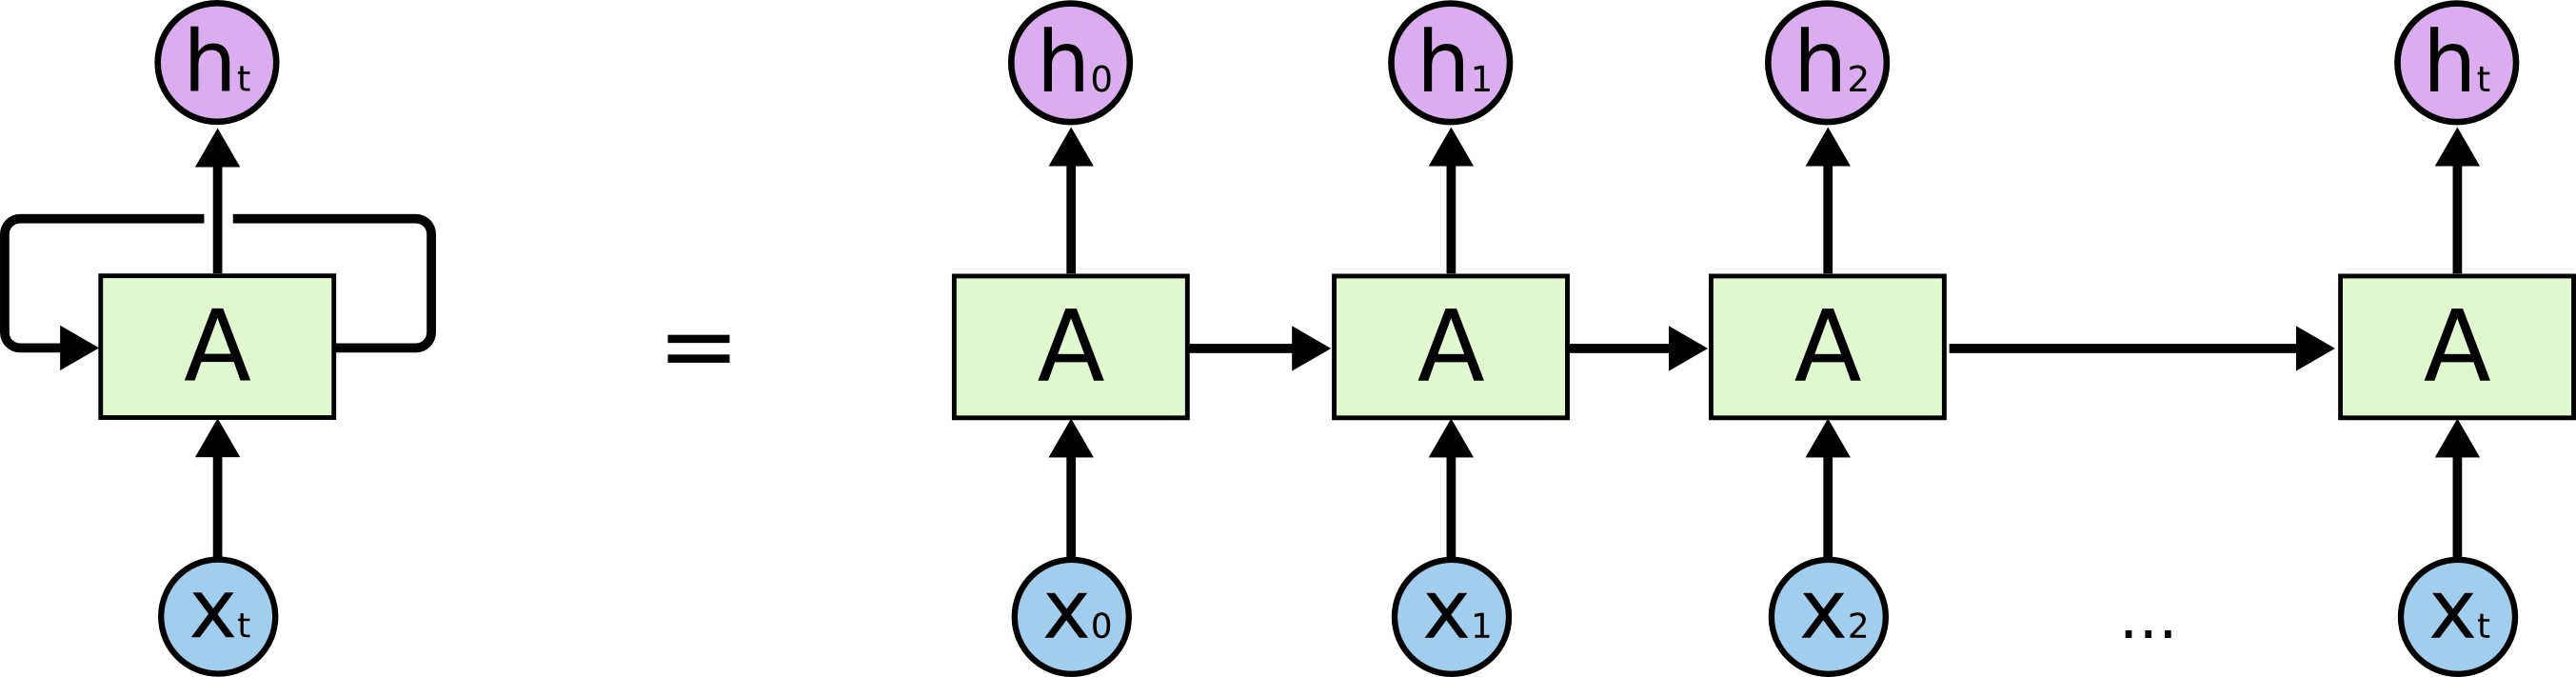
\includegraphics[scale=0.4]{figure/rnn-unroll}
    \caption{Computational graph of Vanilla Recurrent Neural Network on an input sequence\cite{colah-lsmt}.}
    \label{fig:rnn-unfold}
\end{figure}
\label{sec:gradient-vanish}
In theory Vanilla Recurrent Neural Network is Turing-Complete\cite{rnn-turing-complete} but  hard to train (especially on long input sequence) due to the problems of exploding and vanishing gradient\cite{Bengio1994}. 
To scratch the surface, given an output \(h_{t1}\) and a trainable parameter \(W\) at time \(t_2\) which denoted as \(W^{(t_2)}\),  exploding (vanishing) gradient can be understand as the norm \(L2\) of the gradient \(\frac{\partial h_{t1}}{\partial W^{(t_2)}}\) get exponentially bigger (smaller) with respect to the number of time steps \((t_1-t_2)\)\cite{Bengio1994}.
In layman's terms, the longer the dependencies between an output and an input the (exponentially ) harder it is for the training process to capture those dependencies.
This phenomenon is demonstrated in Fig.\ref{fig:gradient-vanish}. 

\begin{figure}[H]
    \centering
    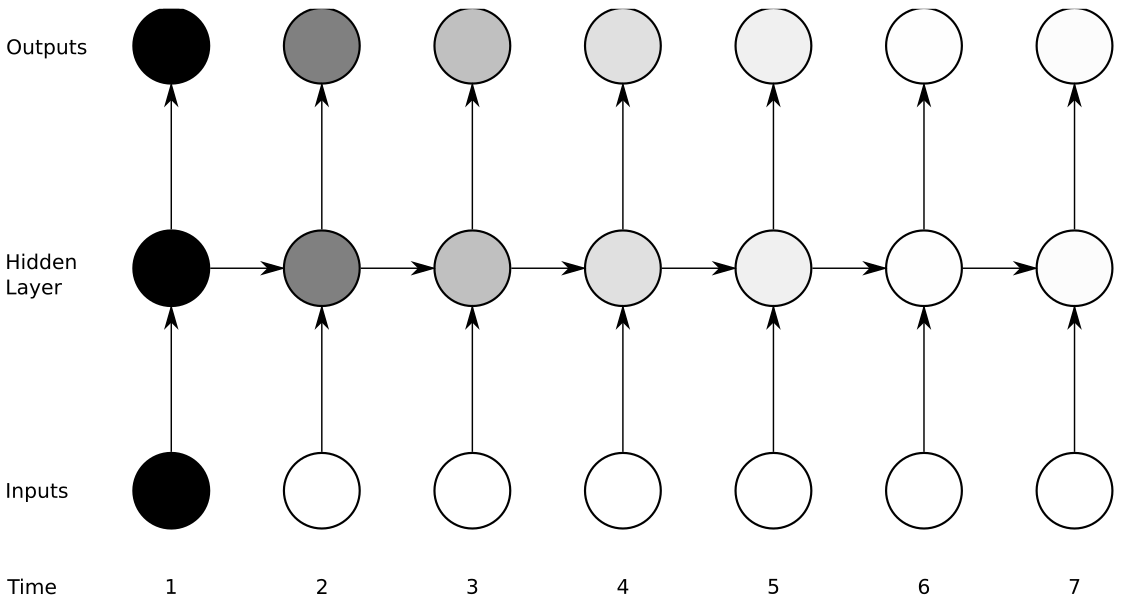
\includegraphics[scale=0.37]{figure/gradient-vanish}
    \caption{Our main focus is on the first input. 
    The shadings on the nodes indicate how much those nodes are affected when the value of the first input changed.
    More technically, denoting the first input as \(i_1\), the shading's intensity of a node \(n\) is calculated as \(\norm{\frac{\partial n}{\partial i_1}}\). 
    The shading's intensity of nodes decrease exponentially through time steps.\cite{Graves-thesis}}
    \label{fig:gradient-vanish}
\end{figure}

For exploding gradient, an ad-hoc technique called gradient clipping\cite{gradient-clip} was introduced and proven to be effective when being applied to many types of RNNs. 
Given a gradient \(G\) that we are going to use to update our parameters, if it norm \(L2\) exceeds a threshold \(m\) we will clip it by this formula:
\begin{align}
      G &:= \frac{Gm}{\norm{G}} &
\end{align}
To mitigate the problem of vanishing gradient, Long Short Term Memory unit (LSTM)\cite{originLSTM} unit was invented. 


\subsubsection{Long Short Term Memory Unit}\label{sec:lstm}
Given a input sequence \(I = (i_0,\ldots,i_n), \forall t, i_t \in \mathbb{R}^n\), Long Short Term Memory unit can be expressed as the following recursive formula\cite{treeLSTM}:
\begin{align}
    w_t &= \sigma(W^{(w)}i_t + U^{(w)}h_{t-1} + b^{(w)}) \label{eq:lstm-input-gate}&\\ 
      f_t &= \sigma(W^{(f)}i_t + U^{(f)}h_{t-1} + b^{(f)}) \label{eq:lstm-forget-gate}&\\ 
      o_t &= \sigma(W^{(o)}i_t + U^{(o)}h_{t-1} + b^{(o)}) \label{eq:lstm-output-gate}&\\ 
      u_t &= tanh(W^{(u)}i_t + U^{(u)}h_{t-1} + b^{(u)}) \label{eq:lstm-update-gate}&\\ 
      c_t &= r_t \otimes u_t + f_t \otimes c_{t-1} \label{eq:longterm-mem}&\\ 
      h_t &= o_t \otimes tanh(c_t) \label{eq:temperal-mem}& 
\end{align}
In the formula above, operator \(\otimes\) is the Hadamard product\cite{element-prod}.
The role of \(h_t\) in LSTM unit is similar to its role in \hyperref[sec:vanilla-rnn]{Vanilla Recurrent unit}. 
Traditionally, \(w_t\), \(f_t\) and \(o_t\) are called input/write gate, forget/deallocate gate and output/read gate respectively. 
In addition, \(c_t\) is called memory cell. 
The output sequence of the LSTM unit is analogous to that of a Vanilla Recurrent unit output sequence \(O = \{h_0,\ldots,h_n\}\).

For intuition, we can interpret how the network works as follow: in the above formula, \(h_{t-1}\) can be view as a short-term memory of the network; \(u_t\) is information extracted from in current input \(i_t\) and the short-term memory \(h_{t-1}\); write gate \(w_t\) decides which information from \(u_t\) will be written into the memory cell \(c_t\); forgot gate \(f_t\) decides which information while be preserved on memory cell \(c_t\); and \(o_t\) decides which information will be read from the memory cell \(c_t\), which will produce the short-term memory (or output) \(h_t\). 
A LSTM illustrated in Fig.\ref{fig:lstm}.

\begin{figure}[H]
    \centering
    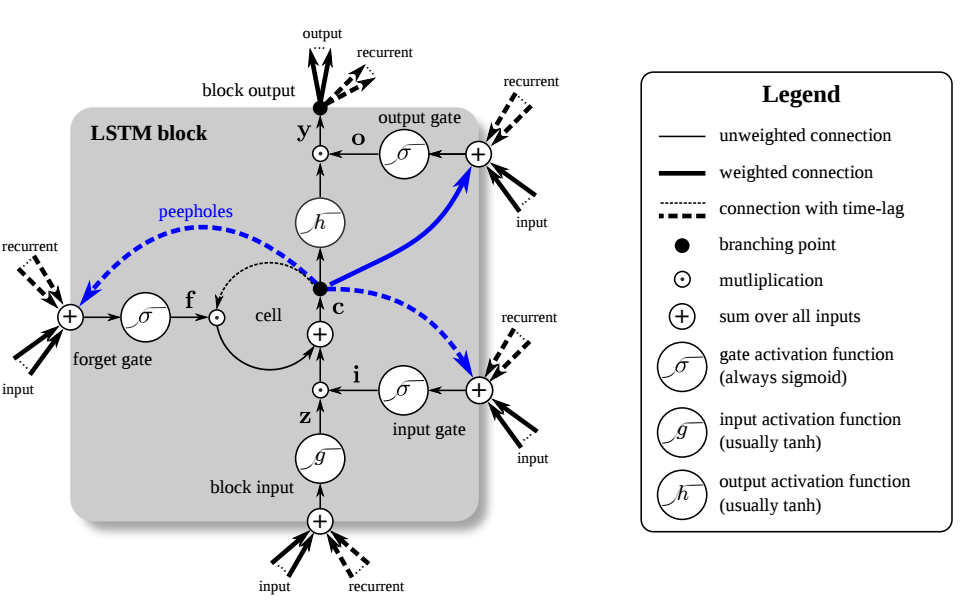
\includegraphics[scale=0.4]{figure/lstm}
    \caption{Diagram of a LSTM unit (exclude blue connections). Blue connections are added in a peephole LSTM.\cite{lstm-search}}
    \label{fig:lstm}
\end{figure}


Other variation on LSTM include adding peephole to three gates of LSTM\cite{peephole} which resulting the following modification\cite{colah-lsmt}:
\begin{align}
    w_t &= \sigma(W^{(w)}i_t + U^{(w)}h_{t-1} + \bm{V^{(w)}c_{t-1}} + b^{(w)}) &\\ 
      f_t &= \sigma(W^{(f)}i_t + U^{(f)}h_{t-1} + \bm{V^{(f)}c_{t-1}} + b^{(f)}) &\\ 
      o_t &= \sigma(W^{(o)}i_t + U^{(o)}h_{t-1} + \bm{V^{(o)}c_{t-1}} + b^{(o)}) &\\ 
      u_t &= tanh(W^{(u)}i_t + U^{(u)}h_{t-1} + b^{(u)}) &\\ 
      c_t &= r_t \otimes u_t + f_t \otimes c_{t-1} &\\ 
      h_t &= o_t \otimes tanh(c_t) & 
\end{align} 

\label{sec:GRU}
Another variation of LSTM unit is GRU unit\cite{GRU}. 
The formula of a  GRU unit can be expressed as follow\cite{colah-lsmt}:
\begin{align}
    z_t &= \sigma(W^{(z)}i_t + U^{(z)}h_{t-1} + b^{(z)}) \label{eq:gru-update}&\\ 
      r_t &= \sigma(W^{(r)}i_t + U^{(r)}h_{t-1} + b^{(r)}) \label{eq:gru-reset}&\\ 
      \tilde{h_t} &= tanh(Wi_t + U(h_{t-1} \otimes r_t) + b) &\\
      h_t &= (1-z_t) \otimes h_{t-1} + z_t \otimes \tilde{h_t} \label{eq:gru-longshort-term}&
\end{align}
Conventionally, \(z_t\) and \(r_t\) were called update gate and reset gate respectively\cite{GRU}. 
In comparison, the role of reset gate \(r_t\) in Eq.\ref{eq:gru-reset} is analogous to the output gate \(o_t\) in a LSTM unit (Eq.\ref{eq:lstm-output-gate}).  
Also, the update gate \(z_t\) in Eq.\ref{eq:gru-update} is the result of constraining the forget gate \(f_t\) to be one minuses the input gate \(i_t\) (in formula: \(f_t = 1-i_t\)) in LSTM unit (Eqs.\ref{eq:lstm-forget-gate},\ref{eq:lstm-input-gate}).
Finally, \(h_t\) (Eq.\ref{eq:gru-longshort-term}) in GRU unit keeps the role of both long-term memory cell \(c_t\) (Eq.\ref{eq:longterm-mem}) and output in a LSTM unit. 
In summarize, GRU unit is a simplified LSTM unit using two ideas: new information overrides old information in memory and the output at a time step is also the current memory cell\cite{evaluate-GRU}.  

Consistently, LSTM and GRU outperform Vanilla RNN in most tasks. 
Intuitively, LSTM or GRU mitigates the problem of vanishing gradient by updating their memory through adding\cite{evaluate-GRU}, although gradients still decrease through time, it is not exponentially\cite{Graves-thesis}. 
In practice, LSTM and GRU performance are comparable and depend on tasks at hand\cite{understand-lstm}\cite{evaluate-GRU}\cite{lstm-search}. 
For that reason, in experiments, we should try both models. 

\subsubsection{Staking Multiple Layers of Recurrent Neural Networks}
Understanding that RNNs can capture long-term dependencies in sequential data, we can amplify this ability by assembling basic RNNs (e.g. Vanilla RNN, LSTM, GRU) to create more sophisticated recurrent architects.
This section introduces several popular combined recurrent architects.
 
For denotation, because all basic recurrent neural networks can be viewed as functions, whose input and output are a sequence of vectors, the forward-pass of any basic RNN model \(r\) can be expressed as \(r(I) = O\) with \(I = \{i_0,\ldots,i_n\}, \forall t, i_t \in \mathbb{R}^n\) and \(O = \{o_0,\ldots,o_n\}, \forall t, o_t \in \mathbb{R}^m\) respectively. 

\paragraph{Multiple Layers Recurrent Neural Networks}\label{sec:multilayer-lstm}
Given a set of basic RNNs \(R = \{r_0,\ldots,r_l\}\), and an input sequence \(I\), a l-layered Recurrent Neural Networks can be presented as the following recursive formula:
\begin{equation}
    \begin{cases}
    O^{(j)} = r_j(O^{(j-1)}), & \mbox{if }  0 < j \leq l\\
    O^{(0)} = r_0(I) 
    \end{cases}
\end{equation}

The output of the system depends on different tasks and setting. 
Denoting the output of the \(j\)th-layer as  \(O^{(j)} = \{o^{(j)}_0,\ldots,o^{(j)}_n\}\), the output can be \(O= \{o^{(0)}_n, o^{(1)}_n\ldots,o^{(j)}_n\}\)\cite{treeLSTM} or \(O = O^{(l)}\) or a combination of both or just \(o^{(l)}_n\). 
An illustration of multi-layer RNN's input, output, and hidden states can be found in Fig.\ref{fig:3-layer-lstm}.

\begin{figure}[H]
    \centering
    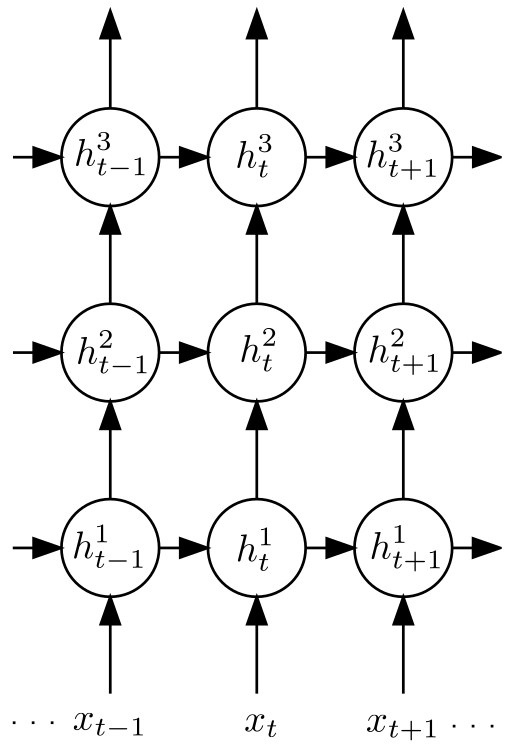
\includegraphics[scale=0.4]{figure/3-layer-lstm}
    \caption{Computational graph of a 3-layer Recurrent Neural Network\cite{GravesLSTM}.}
    \label{fig:3-layer-lstm}
\end{figure}

This type of recurrent models were applied in multiple researches\cite{GravesLSTM}\cite{SutskeverVL14}\cite{ZarembaS14}\cite{treeLSTM}.
Recurrent models with more layers might have the ability to capture longer-term dependency\cite{treeLSTM}.
In practice, the number of layers \(l\) is treated as hyper-parameter.

\paragraph{Bidirectional Recurrent Neural Networks}\label{sec:bilstm}
In some sequential data prediction problem, an output does not only depend on the input sequence before it but also the input sequence after it. 
Addition, some dependencies are easier to capture when the input is processed in reverse order.
In those cases, Bidirectional Recurrent Neural Networks might have advantages over the basic RNNs\cite{GravesLSTM}\cite{Graves-thesis}.

Given an input sequence \(\overrightarrow{I} = \{i_0,\ldots,i_n\}\), we define the reverse input sequence of \(\overrightarrow{I}\) as \(\overleftarrow{I} = \{j_0,\ldots,j_n\}\) with \(j_t = i_{n-t}\). 
Using two RNNs \(r_0\) and \(r_1\), the formula of Bidirectional Recurrent Neural Networks can be expressed as follow:
\begin{align}
    \overrightarrow{O} &= r_0(\overrightarrow{I}) &\\
    \overleftarrow{O} &= r_1(\overleftarrow{I}) &
\end{align}
\(\overrightarrow{O}\) and \(\overleftarrow{O}\) can be combined in different ways depend on tasks and settings\cite{GravesLSTM}\cite{Graves-thesis}\cite{treeLSTM}.

\begin{figure}[H]
    \centering
    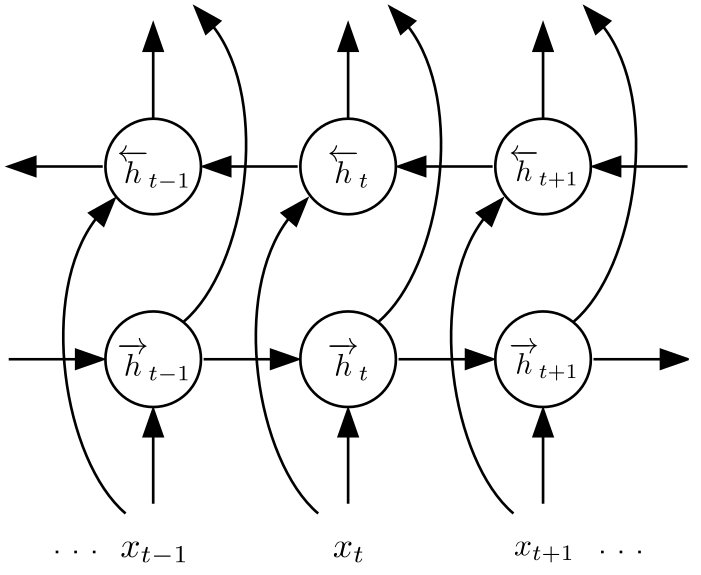
\includegraphics[scale=0.4]{figure/blstm}
    \caption{Computational graph of a Bidirectional Recurrent Neural Network\cite{GravesLSTM}.}
    \label{fig:blstm}
\end{figure}

\paragraph{Multiple Layers Bidirectional Recurrent Neural Networks}
Given any Recurrent architects \(r\), we can define two operations on it: bidirectional operation \(B(r)\) and multi-layer operation \(M(r, l)\) with \(l\) as the number of layers added.
Using these operators, we can assemble an infinite number of new recurrent architects. 
For example the architects illustrated in Fig.\ref{fig:dblstm} can be expressed as \(M(B(lstm), 2)\).

\begin{figure}[H]
    \centering
    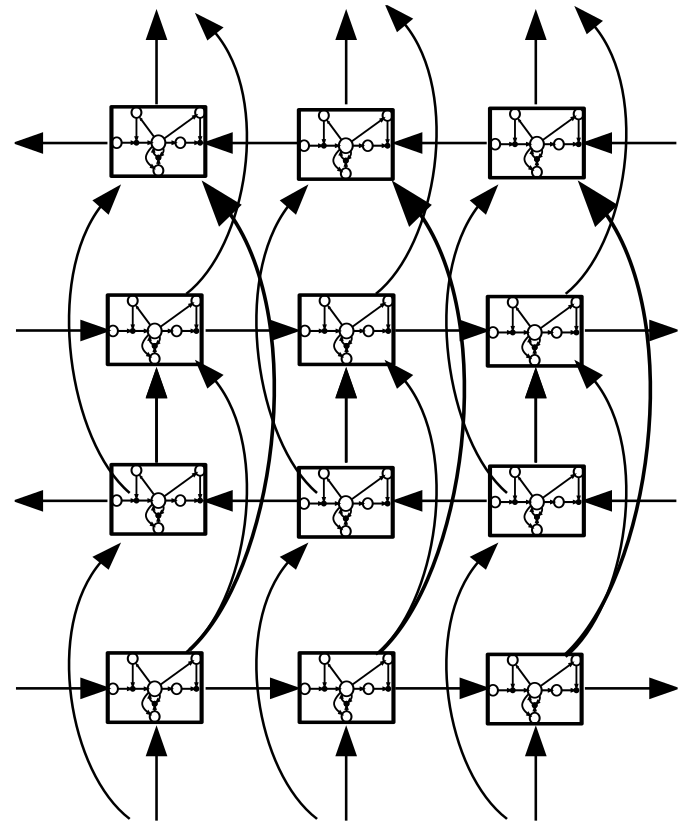
\includegraphics[scale=0.4]{figure/dblstm}
    \caption{Computational graph of a Deep Bidirectional Recurrent Neural Network\cite{GravesLSTM}.}
    \label{fig:dblstm}
\end{figure}

\subsection{Improved Semantic Representations From Tree-Structured Long Short-Term Memory Networks (Tree-LSTMs)}\label{sec:treelstm}
Compare to other network architects, Recurrent Neural Network have a great advantage in handling sequential, arbitrary length input (e.g. sentences, paragraphs, a sequence of frame in a video or a sequence of acoustic unit in a spoken word) but on the other hand, it also comes with the disadvantage of being hard to train\cite{hardRNN}.
Given a sequence of input, the network has to capture features which can be long-range relationships between inputs\cite{socher2013recursive}.
One way to improve such structure would be to make these features easier to capture, in other words, shorten the length of relationships between inputs.
For the case of sentences, we can present them as syntactic parse trees, in which relevant words and phrases are presented closer to each other in an intuitive way (as human, we understand sentences base on phased and phrases base on words). 
In this paper\cite{treeLSTM}, the authors explored this idea by using tree-structured LSTM to combine sentence presentation from its words.
They archive state-of-the-art performance on two tasks: predicting the semantic relatedness of two sentences (SemEval 2014, Task 1\cite{SemeEvalTask1}) and sentiment classification (Stanford Sentiment Treebank\cite{socher2013recursive}).


Given the advantages of tree structure over it sequential counterpart, we will apply this theory to our model in \hyperref[sec:VTtree]{4.1.1} and \hyperref[sec:CNNtree]{4.1.2}. 
Their experiments were originally implemented in \hyperref[sec:torch]{Torch7}\footnote{\url{https://github.com/stanfordnlp/treelstm}}, for the purpose of extending their models and doing more experiments, we re-implemented\footnote{\url{https://github.com/ttpro1995/TreeLSTMSentiment}} their models in \hyperref[sec:pytorch]{PyTorch}. 

As we only interested in the task of sentiment analysis, the experiment and result which related to the task of semantic relatedness will not be presented.

\subsubsection{Method}
\paragraph{Child-Sum Tree-LSTMs}
Given a tree, we denote \(C(j)\) as set of children of node \(j\).
The step of calculation inside Child-Sum Tree-LSTM node \(j\) can be expressed as follow\cite{treeLSTM}:
\begin{align}
      \tilde{h_j} &= \sum_{k \in C(j)} h_k &\label{eq1:2}\\
      i_j &= \sigma{(W^{(i)}x_j + U^{(i)}\tilde{h_j} + b^{(i)})} &\label{eq1:3}\\
      f_{jk} &= \sigma{(W^{(f)}x_j + U^{(i)}h_k + b^{(f)})}, \qquad  \forall k \in C(j) & \label{eq1:foget1}\\
      o_j &= \sigma{(W^{(o)}x_j + U^{(o)}\tilde{h_j} + b^{(o)})} &\label{eq1:5}\\
      u_j &= \tanh{(W^{(u)}x_j + U^{(u)}\tilde{h_j} + b^{(u)})} &\label{eq1:6}\\
       c_j &= i_j \odot u_j + \sum_{k \in C(j)} f_{jk} \odot c_k & \\
    h_j &= o_j \odot \tanh{(c_j)} &
\end{align}

As Child-Sum Tree-LSTMs has the ability to combine node with an arbitrary number of children, it is can be applied to compose sentence based on it dependency parse tree.
This application was named by the authors as \textbf{Dependency Tree-LSTMs}\cite{treeLSTM}.

\paragraph{N-ary Tree-LSTMs}
Given a tree, we denote \(C(j)\) as the set of children of node \(j\) and \(N\) as the maximum number of children a node can have. 
We will assume that the number of child in a node is always \(0\) or \(N\). 
If a node has no children nodes, we call it a leaf-node, else, it will be called a composer-node. 

The calculation steps inside leaf-node (leaf-module) \(j\) can be expressed as follow:
\begin{align}
    o_j &= \sigma{\left( W^{(o)} x_j + a^{\left(o\right)}\right)} & \\
       c_j &= W^{(c)} x_j + a^{(c)} & \\
    h_j &= o_j \odot \tanh{\left(c_j\right)} &
\end{align}

The calculation steps inside composer-node (composer-module) \(j\) can be expressed as follow:
\begin{align}
      i_j &= \sigma{ \left(\sum_{l=1}^{N}U_l^{(i)} h_{jl} + b^{(i)} \right) } &\label{eq:9}\\
      f_{jk} &= \sigma{\left(\sum_{l=1}^{N}U_{kl}^{\left(f\right)} h_{jl} + b^{\left(f\right)}\right)}, \qquad  \forall k \in C(j) & \label{eq:foget2}\\ 
      o_j &= \sigma{\left( \sum_{l=1}^{N}U_l^{\left(o\right)} h_{jl} + b^{\left(o\right)}\right)} &\label{eq:11}\\
      u_j &= \tanh{\left( \sum_{l=1}^{N}U_l^{\left(u\right)} h_{jl} + b^{\left(u\right)}\right)} &\label{eq:12}\\
       c_j &= i_j \odot u_j + \sum_{k \in C\left(j\right)} f_{jk} \odot c_{jl} & \\
    h_j &= o_j \odot \tanh{\left(c_j\right)} & \\
\end{align}

Different from Child-Sum Tree-LSTMs forget gate in Eq.\eqref{eq1:foget1}, N-ary Tree-LSTMs chooses what to forget based on all it children as in Eq.\eqref{eq:foget2}. 
Also, each the combination of \(h_{jl}\) in Eqs.\eqref{eq:9},\eqref{eq:11}, \eqref{eq:12} are parameterize by \(U_l^{(i)}\), \(U_l^{(o)}\) and \(U_l^{(u)}\) respectively, compares to linear transformation of sum (Eqs.\eqref{eq1:2}, \eqref{eq1:3}, \eqref{eq1:5}, \eqref{eq1:6}) in Child-Sum Tree-LSTMs.

Knowing that any constituency parse tree can always be presented in a binarized form, to compose a sentence the authors applied 2-ary Tree-LSTMs on the binarized constituency parse tree of that sentence. 
This combination was named by the authors as \textbf{Constituency Tree-LSTMs}\cite{treeLSTM}.

\paragraph{Output module} Denoting sequence of words spanned by a sub-tree rooted at node \(j\) as \(\{x\}_j\). 
For both Dependency Tree-LSTMs and Constituency Tree-LSTMs when applying on the task of sentiment analysis, the prediction at node \(j\) can be computed by an output-module as follow\cite{treeLSTM}:

\begin{align}
      \hat{p_{\theta}}(y \mid \{x\}_j ) &= softmax( W^{(s)} h_j + b^{(s)}) & \\
      \hat{y_j} &= \underset{y}{\mathrm{argmax}} \; \hat{p_{\theta}}(y \mid \{x\}_j ) &
\end{align}

The authors use negative log-likelihood with \(L2\) regularization as loss function\cite{treeLSTM}.

\paragraph{Training technique and hyper-parameters}
Glove vectors\cite{glove} was used to initialize word-embedding. 
The words presentation were updated with learning rate 0.1 while other parameters in the network were update using AdaGrad\cite{adagrad} with learning rate 0.05. 
Batch-size was set to 25. 
\(L2\) regularization was applied at each mini-batch with weight of \(10^{-4}\).
The authors also added a dropout layer\cite{dropout} with dropout rate of \(0.5\) before each output-module.

\subsubsection{Results and Discussion}
\begin{table}[H]
\centering
\begin{tabular}{l c} 
 \hline
 \hline 
 Method & Accuracy \\ [0.5ex] 
 \hline
 \hline
 \\  
 RAE\cite{socher2013recursive} & 82.4 \\ 
 MV-RNN\cite{socher2013recursive} & 82.9 \\
 RNTN\cite{socher2013recursive} & 85.4 \\
 DCNN\cite{DCNN} & 86.8 \\
 Paragraph-Vec\cite{ParagraphVec} & 87.8 \\
 CNN-non-static\cite{KimCNN} & 87.2 \\
 CNN-multichannel\cite{KimCNN} & 88.1 \\
 DRNN\cite{IrsoyDRNN} & 86.6 \\ [0.5ex]
 \hline
 \\  
 LSTM\cite{originLSTM} & 84.9 (0.6) \\ 
 Bidirectional LSTM\cite{GravesLSTM} & 87.5 (0.5) \\
 2-layer LSTM\cite{GravesLSTM} & 86.3 (0.6) \\
 2-layer Bidirectional LSTM\cite{GravesLSTM} & 87.2 (1.0) \\ [0.5ex]
 \hline 
 \\  
 Dependency Tree-LSTM\cite{treeLSTM} & 84.9 (0.6) \\ 
 Constituency Tree-LSTM\cite{treeLSTM} &  \\ 
 \; with randomly initialized vectors & 82.0 (0.5) \\ 
 \; Glove vectors, fixed & 87.5 (0.8) \\
 \; Glove vectors, tuned & 88.0 (0.3) \\
 \hline
 \hline
\end{tabular}
\caption{Test set accuracies on Stanford Sentiment Treebank with binary setting.
In the first block, the results were reported in their original papers. 
The second block contains results produced by sequential models and tree-structured models for the third block. 
For each models in the second and third block, mean accuracy over 5 runs (standard deviation in parentheses) was reported}
\label{table:1}
\end{table}

The results presented in Table\ref{table:1} support the hypothesis that tree-structured LSTMs are better than sequential LSTMs when applying on sequences which have nested grammar\cite{treeVSseq}. 
We should notice that good word embedding give a great boost to the system\cite{Luong_betterword}, fine-tune also beneficial.

\begin{figure}[H]
    \centering
    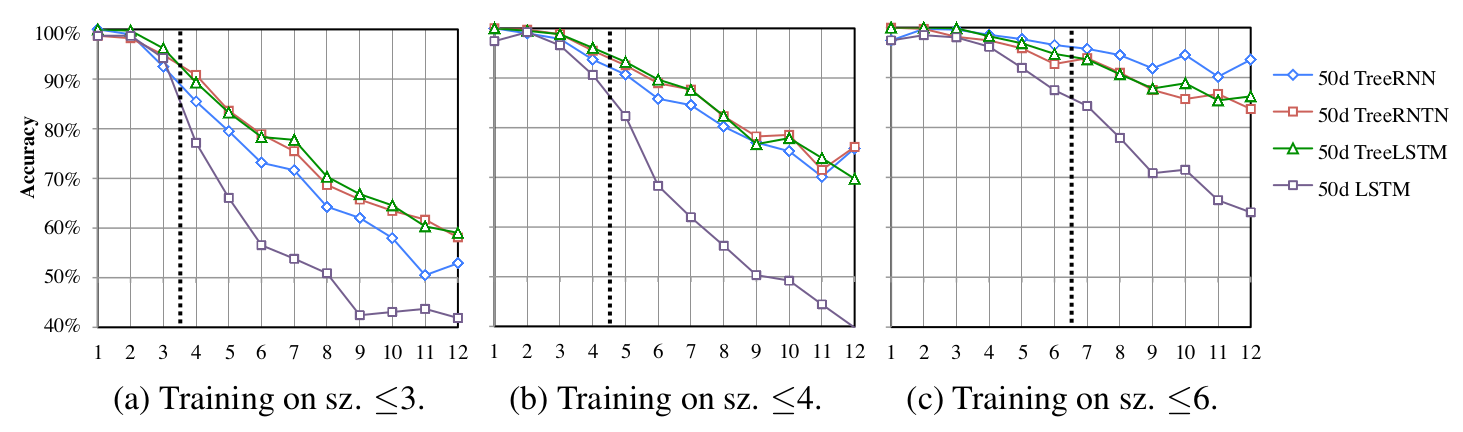
\includegraphics[scale=0.405]{figure/tree-vs-seq}
    \caption{Test accuracy on three experiments with increasing limited length of sentences in training data. 
The vertical axis is accuracy and the horizontal axis is limited length of sentences in testing data. 
Experiments were done with \cite{socher2013recursive}, TreeRNTN\cite{socher2013recursive}, TreeLSTM\cite{treeLSTM} and LSTM\cite{originLSTM}. 
50 is the number of dimension of hidden stat \(h\). 
This data set was generated using an artificial recursively defined language\cite{bowman-treevslstm}.} 
    \label{fig:tree-vs-seq}
\end{figure}
\label{sec:tree-discuss}
\textbf{Advantages of Tree-LSTMs} are presented in several studies\cite{need-tree}\cite{bowman-treevslstm}: \label{treelstm-advantage}
\begin{itemize}
\item In case the input sequence belong to recursively defined language, given only a small subset of the data with limited length sentences, tree structures model have better ability to generalize compare to sequential ones.
But when we increase the limited length sentences, the advantage of tree over sequential models decrease fast\cite{bowman-treevslstm}. 
This can be demonstrated in Fig.\ref{fig:tree-vs-seq}.
\item Tree can break down complicated sentences into simpler phrases, which make it easier for generalization\cite{improve-presentation}\cite{need-tree}.
\item Some features which are far apart when a sentence is presented as sequence become closer when it is presented as tree\cite{need-tree}.
\end{itemize}


\textbf{Disadvantages of Tree-LSTMs} including:\label{treelstm-drawback}
\begin{itemize}
\item Sentences can be wrongly parsed, especially when comments are expressed in informal language.
The performance of the system depended on the parser being used.
\item When combining a sub-tree, that sub-tree have no information about its context. 
Compared to sequential structures, when combining an input (e.g. word, phrase), the network already has the left context information of that input\cite{shift-reduce}.
\item A closer look at Eqs.\eqref{eq1:6},\eqref{eq:12} reveal that, Tree-LSTMs have only a logistic regression at each node to capture features.
We think this is the reason why Kim's CNN\ref{kim-cnn} can outperform TreeLSTMs.  
\item Tree-LSTMs can not be trained using batch in parallelism. But this disadvantage can be overcome thank to Tree-LSTMs shift-reduce implementation\cite{shift-reduce}.
\end{itemize}


\subsection{Convolutional Neural Networks for Sentence Classification}\label{kim-cnn}
In Table\ref{table:1}, we can see that the best model is not Constituency Tree-LSTM but CNN-multichannel\cite{KimCNN}, which was originally presented in this paper. 
With only a one-layer \hyperref[sec:cnn]{Convolution Neural Network}, and general hyper-parameter tuning, the author was able to archive state-of-art\footnote{in 2014} performance on several NLP tasks, which include sentiment analysis (\hyperref[sec:sst]{Stanford Sentiment Treebank}\cite{socher2013recursive}). 
The paper also successfully adapted the idea of training CNN on multiple channels image in Computer Vision to training CNN on multi-channel words embedding for sentence\footnote{Implementation of this paper can be found at \url{https://github.com/yoonkim/CNN\_sentence}}.

\begin{figure}[H]
    \centering
    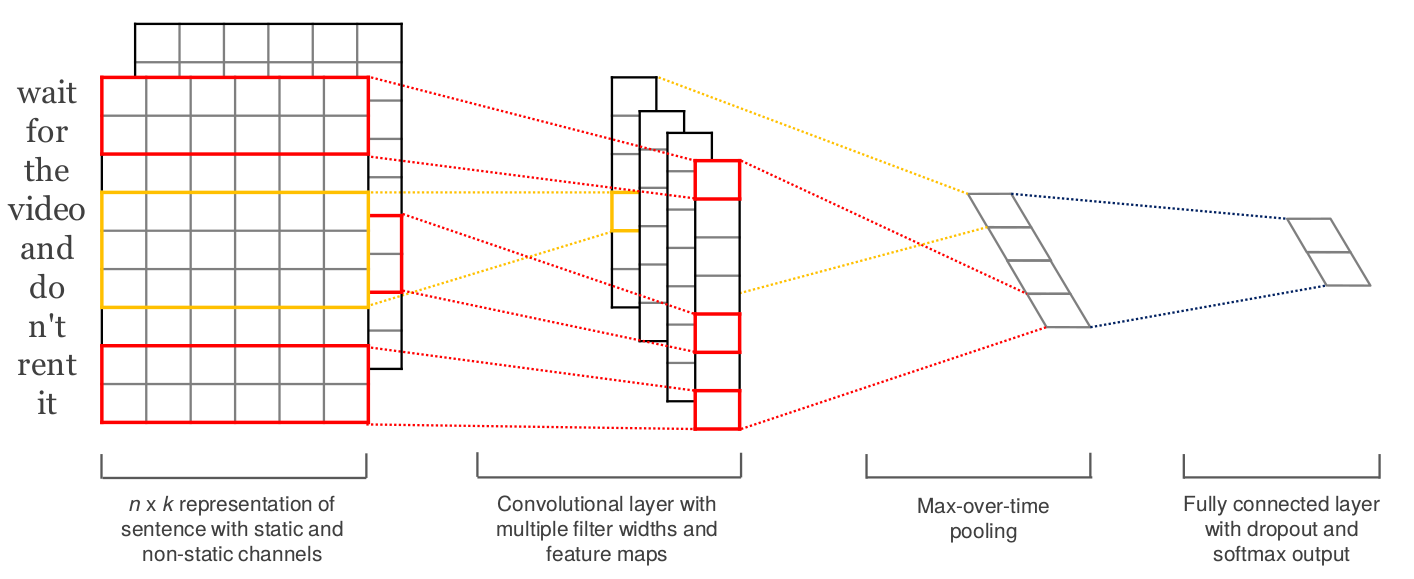
\includegraphics[scale=0.33]{figure/sentencecnn}
    \caption{Structure of CNN with two word embedding channels of the same sentence}
    \label{fig:multi-cnn}
\end{figure}

\subsubsection{Method}
Let denote \(\bm{x_i \in \mathbb{R}^d}\) as a \(d\)-dimension vector presentation of word-\(i\)th in a sentence. 
Given a sentence \(\bm{s}\) of length \(n\), we can present a sub-sequence of words in the sentence which start at word-\(i\)th and end at word-\(j\)th as:
\begin{align}
    x_{i:j} &= x_i \oplus x_{i+1} \oplus ... \oplus x_{j} &\label{concat}
\end{align}
In Eq.\eqref{concat}, operator \(\bm{\oplus}\) do concatenation. Therefore, \(x_{i:j} \in \mathbb{R}^{d(j-i+1)}\). 

\paragraph{Convolution filter} \label{conv-filter} Now we are ready to define a filter. A filter with window size \(\bm{l}\) is a vector \(\bm{w \in \mathbb{R}^{ld}}\) which apply on vector presentations of word-\(i\)th to word-\((i+l-1)\)th through the following equation:
\begin{align}
    c_i &= f(w \cdot x_{i:i+l-1} + b) &\label{filter}
\end{align}

In Eq.\eqref{filter}, \(\bm{b \in \mathbb{R}}\) as bias term and \(\bm{f}\) is a activation function. 

\begin{figure}[H]
    \centering
    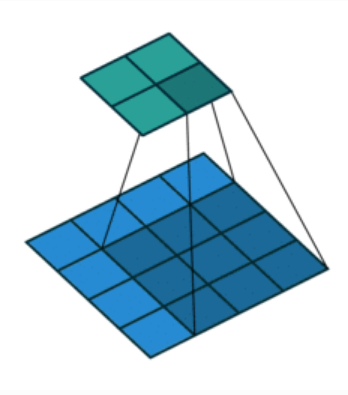
\includegraphics[scale=0.4]{figure/no_padding}
    \caption{No padding and unit strides policy when applying a filter on a matrix.}
    \label{fig:no_padding}
\end{figure}

By slicing the filter through the sentence we can get vector \(\bm{c}\) which can be view as a feature map of sentence \(s\). 
In this paper, the author use no padding and unit strides policy (Fig.\ref{fig:no_padding}), which gives \(c \in \mathbb{R}^{n-l+1}\).

\paragraph{Max-over-time pooling}\label{sec:max-overtime-pooling} Given the feature map, the author then take the maximum value in it \(\bm{c^* = max\{c\}}\) (max-over-time pooling\cite{nlp-scratch}), which is a sentence feature produced by the filter.
So, convoluting a filter with the sentence will produce one feature \(\bm{c^* \in \mathbb{R}}\).

\paragraph{Sentence presentation} Applying \(\bm{k}\) filters on the sentence, and we will have a feature vector \(\bm{p \in \mathbb{R}^k}\). 
In case of sentiment classification, the feature vector \(p\) can be fed to a classifier like the one in the last layer of the architect presented in Fig.\ref{fig:multi-cnn}.

\paragraph{Multi-channel input} Given that the sentence is presented by a set of channels \(\bm{Z}\) and the network has \(\bm{k}\) filters. 
We will modify Eq.\eqref{filter} as follow: 

\begin{align}
    \forall h \in Z, \; \; \hat{c}_{ih} &= f(w \cdot x_{i:i+l-1} + b)& \\
    c_i &= \sum_{h \in Z} \hat{c}_{ih}&
\end{align}

The rest of the system is unchanged compared to a single-channel one.
The whole process is illustrated in the first two layers of the architect in Fig.\ref{fig:multi-cnn}.

\paragraph{Experimented models} The author did experiments with several variations:

\begin{itemize}
      \item \textbf{CNN-rand:} One channel word embedding are randomly initialized and updated during the training process.\label{cnn-rand}
    \item \textbf{CNN-static:} One channel word embedding are initialized with word2vec\cite{word2vec} and not updated during the training process even for unknown randomly initialized new word.\label{cnn-static}
    \item \textbf{CNN-non-static:} One channel word embedding are initialized with word2vec and updated during the training process.\label{cnn-non-static}
    \item \textbf{CNN-multichannel:} Two channels word embedding are initialized with word2vec. One of the channel is updated during the training process the other is kept static.\label{cnn-multichannel}
\end{itemize}
\paragraph{Training method and hyper-parameters} 
Rectifier\cite{rectifier} were use as activation function.
The author used window size 3, 4 and 5, each of which have 100 filters, the max-over-time pooling layer will produce a 300-dimension sentence presentation vector. 
Dropout layer was used after the max-over-time pooling layer with dropout-rate of \(0.5\).  
Batch-size was set to 50. 
All weight vectors were normalized to have \(\norm{w}_2 = 3\) whenever \(\norm{w}_2 > 3\). 
Adadelta\cite{adadelta} was used as optimizer of the networks.
When training on Stanford Sentiment Treebank, each labeled sub-tree's span was treated as an example.
At test phase, each input is a sentence, and output is a sentiment prediction for that sentence.

\subsubsection{Results and Discussion}\label{kimcnn-drawback}
\begin{table}[H]
\centering
\begin{tabular}{l c} 
 \hline
 \hline 
 Method & Accuracy \\ [0.5ex] 
 \hline
 \hline
 \\  
 CNN-rand & 82.7 \\ 
 CNN-static & 86.8 \\ 
 CNN-non-static & 87.2 \\ 
 CNN-multichannel & 88.1 \\ 
 \hline
 \hline
\end{tabular}
\caption{Test set accuracies on Stanford Sentiment Treebank with binary setting. These models are presented in\ref{cnn-multichannel}.
A comparison with models from different works has been presented in\ref{table:1}}
\label{table:KimCNN}
\end{table}

Multiple channels with one static and one for fine-tuning help the network to better generalize.
There is a drawback in CNN-multichannel: although max-over-time pooling largely simplified the network (which is good for preventing over-fit), it only tell if a feature appears in a sentence or not, the information about position of the feature is ignored.\label{kim-drawback}
The next research in\ref{cnn-rnn}  improve CNN-multichannel based on this drawback.
 

\subsection{Combination of Convolutional and Recurrent Neural Network for Sentiment Analysis of Short Texts (CNN-RNN)}\label{cnn-rnn}
As we have observed the drawback of max-over-time pooling layer in\ref{kimcnn-drawback}, we will analyze how the authors of this paper\cite{cnn-rnn} tackled it.

\subsubsection{Method}
\begin{figure}[H]
    \centering
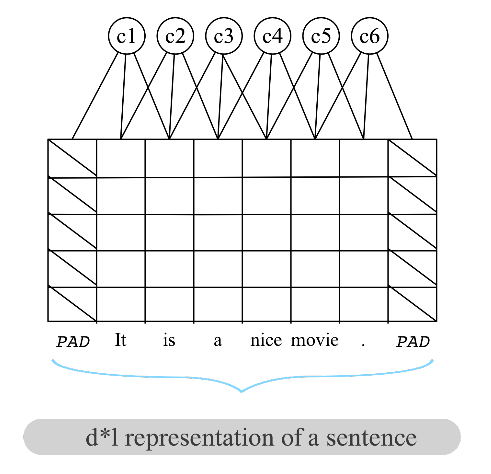
\includegraphics[scale=0.45]{figure/conv-word}
    \caption{A convoluting filter slicing through a sentence. 
    Padding was added.}
    \label{fig:conv-word}
\end{figure}

\paragraph{Preprocessing Sentence} We re-use the definition of convolution filter described in\ref{conv-filter}.
Given a sentence \(s\), the authors first padding it with \((l-1)\) "dummy-words" on each end of the sentence, with \(l\) as the largest window size among all filters.
After that, the padded-sentence is padded on its right until reaching the length of the longest padded sentence in the data set.
In other words, given that \(m\) is length of the longest sentence in SST, the input of a filter with window size \(l\) will always be a padded-sentence of length \((m + 2(l-1))\).
A filter of size \(k\) than slice through a padded-sentence with unit strides and product a feature map \(c \in \ \mathbb{R}^{m + 2l - k - 1}\).
This process in illustrated in Fig.\ref{fig:conv-word}

\begin{figure}[H]
    \centering    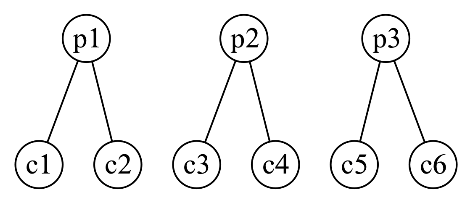
\includegraphics[scale=0.34]{figure/2-max}
    \caption{Max pooling with window size 2 and strides 2 slicing through a feature map}
    \label{fig:2-max-pooling}
\end{figure}
  
\paragraph{Max pooling layer} A max pooling layer of window size 2, with strides 2, slice through each feature map, and reduce its size by a half.
We will denote this vector \(p \in \mathbb{R}^{\floor{\frac{m + 2l - k - 1}{2}}} \). 
This process in illustrated in Fig.\ref{fig:2-max-pooling}   


\begin{figure}[H]
    \raggedleft    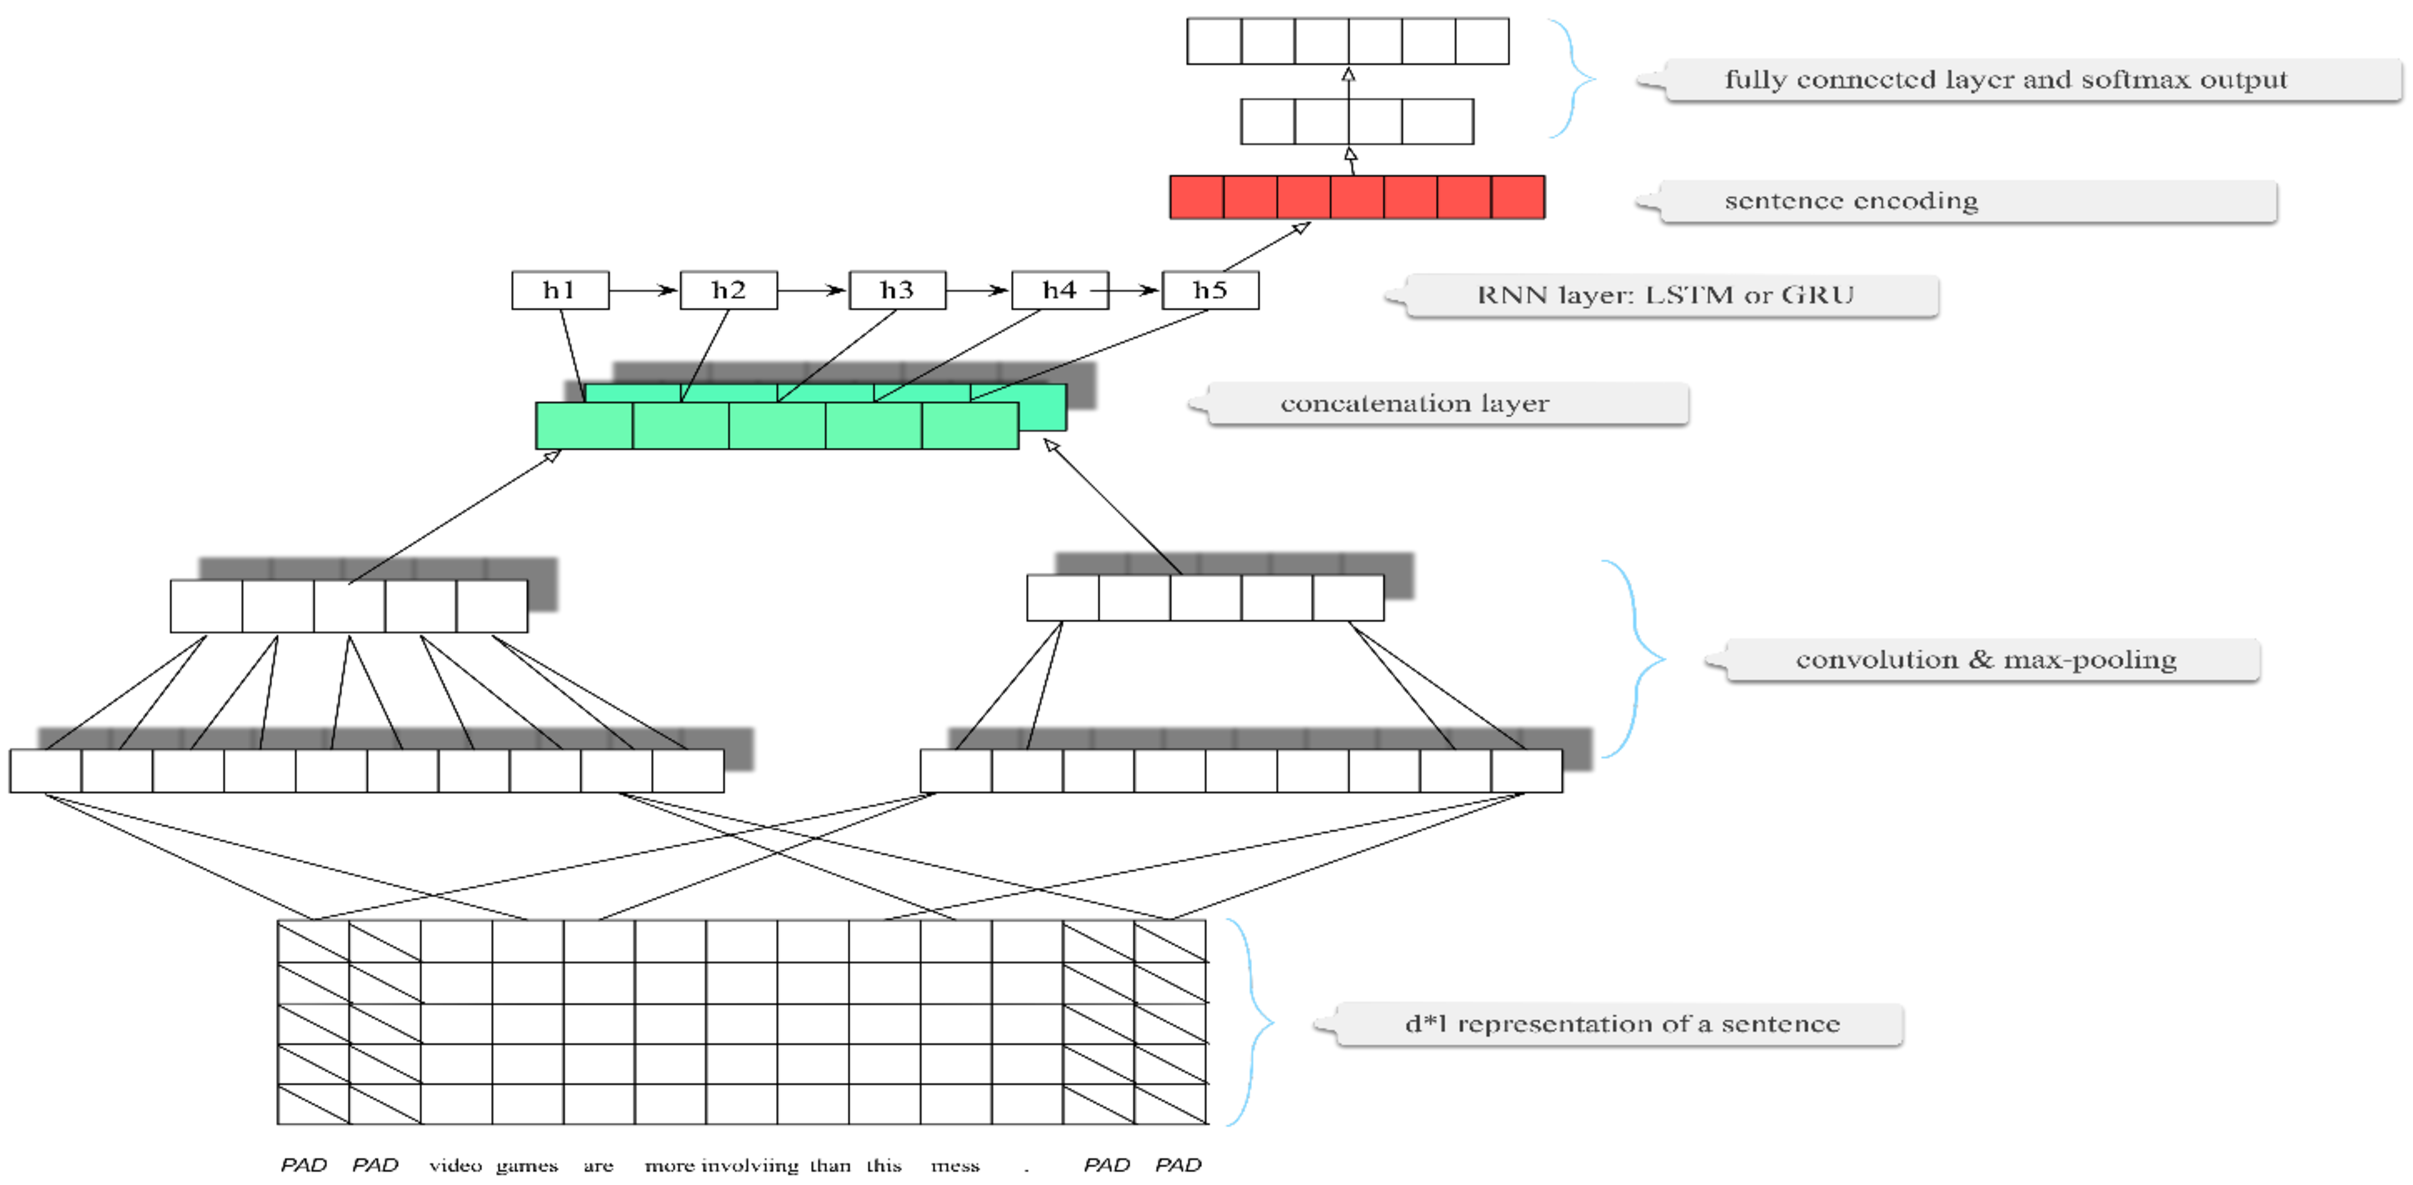
\includegraphics[scale=0.425]{figure/cnn-rnn}
    \caption{CNN-RNN}
    \label{fig:cnn-rnn}
\end{figure}

Note that for filters with different window sizes, the size of feature vectors \(p\) are also different. 
This will be problem if we want to compile feature vectors with different size.
To solve this problem, the authors chose only two types of window size: \(4\) and \(5\).
Which results in all feature vectors having the same size. 

Suppose we have \(n\) filters, authors then concatenated all the feature vectors into one matrix \(P \in \mathbb{R}^{n \times \floor{\frac{m + 2l - k - 1}{2}}}\), which each row is a feature vectors. 
After that, each column in \(P\) treated as an input \(i \in \mathbb{R}^{n}\) for a recurrent neural network, which can be RNN, LSTM or GRU.
The last output the recurrent neural network can be then fed to MLP for classification.
The whole process is demonstrated in Fig.\ref{fig:cnn-rnn}.

\paragraph{Training method and hyper-parameters} 
Word presentation vectors were initialized with word2vec\cite{word2vec}.
The author used window size 4 and 5, each of which has 200 filters. 
When training on Stanford Sentiment Treebank, each labeled sub-tree's span was treated as an example.
At test phase, each input is a sentence, and output is a sentiment prediction for that sentence.
Other hyper-parameters were not specified in this paper, but can be found in the authors' implementation\footnote{\url{https://github.com/ultimate010/crnn}}.

\subsubsection{Results and Discussion}
\begin{table}[H]
\centering
\begin{tabular}{l c} 
 \hline
 \hline 
 Method & Accuracy \\ [0.5ex] 
 \hline
 \hline
 \\  
 MAX-GRU & 89.95 \\ 
 MAX-LSTM & 89.56 \\ 
 AVG-GRU & 89.61 \\ 
 \hline
 \hline
\end{tabular}
\caption{Test set accuracies on Stanford Sentiment Treebank with binary setting. 
The models' names have the following format: \{type pooling layer\}-\{type of RNN\}.
A comparison with models from different works has been presented in\ref{table:1}}
\label{table:cnn-rnn}
\end{table}

This paper proved that the ability to combine feature based on their position is important for sentence-level sentiment analysis. 
This is one way to overcome the disadvantage in Yoon Kim's models\ref{kim-drawback}.


\subsection{Unsupervised pre-training models}\label{sec:unsupervised-pretrain}
A large number of studies have prove that unsupervised pretraining model can help it greatly generalize\cite{why-unsupervised}\cite{greedy-layer}\cite{greedy-layer-bengio}\cite{pretrain-1}.
In case of Sentiment Analysis and specifically the task on Stanford Sentiment Treebank, we can identify several challenges that can be overcome using unsupervised pre-train technique\cite{why-unsupervised}:
\begin{itemize}
\item Given the training data set of SST, the network have no knowledge about film industry (e.g. movie genres, director, actor, art style). 
\item It also does not know human emotions or meaning of their expressions.
\item The network also have little knowledge about meaning of phrases, idioms, meaning of words based on its' context.
\item The network might have too many tuning parameters compare to the number of training examples in SST. 
Which can lead to over-fitting.
\end{itemize}
We will present several potential methods that are applicable for our models. 

\subsubsection{Natural Language Modeling}\label{sec:nlm}
The goal of language modeling is to model the probability distribution of a word conditioning on the words before it.
More concretely, given a sequence of words (or history) \((w_0, w_1,\ldots,w_n)\), the task of a language model \(M\) is to model the probability distribution \(P_M(w_{n+1}|w_0, w_1,\ldots,w_n)\). 
For this task, we can use any model (e.g. recurrent neural network, convolution neural network, MLP) that have the ability to encode an arbitrary sequence of words/symbols (belong to our language).
The encoded context is then used to predict the next word \(w_{n+1}\).
With consideration, the whole system can be trained end-to-end.\footnote{Pytorch implementation: \url{https://github.com/pytorch/examples/tree/master/word\_language\_model}}

We can evaluate a language model by measuring its perplexity on a test data set. Given test data \(T = (w_0, w_1,\ldots,w_n)\), the perplexity \(PP_T\) of a model \(M\) on \(T\) can be calculated as follow\cite{perplexity}:
\begin{align}
    PP_T(M) &= \frac{1}{\sqrt[n]{\prod_{i=0}^{n} P_M(w_{i}|w_0, w_1,\ldots,w_{i-1})}}&
\end{align}

\textbf{The advantages} of this approach including:
\begin{itemize}
\item Can be trained on a large number of data sets, with the only condition those the data sets belong to the language.
\item If we pre-train our models on Amazon Reviews data set, the models can learn to capture sentiment features, as it needs to predict the distribution of words in comments.
It could also learn more interesting features, such as: 
The reviewer cries when watching a good romantic movie, or the viewer praises the novel and then criticizes the movie based on the novel, or how sentiments being expressed by sentence structures. 
This technique has been reported to improve accuracy on Rotten Tomatoes sentiment classification task\cite{Rotten-Tomato} (which is a super set of Stanford Sentiment Treebank data set(Sec.\ref{sec:sst})).
\end{itemize}

One clear disadvantage of this approach is that we can not use it to unsupervised pre-train tree structured networks. 
As tree need full sentence with or full phrase, it can not process arbitrary words sequence. 

\subsubsection{Sentence Encoding}
In this approach, the whole sentence is encoded using some models that we wish to pre-train. 
The encoded sentence is then used to predict the words it contains.  
The prediction task can be defined in different ways:
\begin{itemize}
\item We can use a small context window around the guesting word.
The words in context window and vector presentation of the sentence can be concatenated/averaged and feed to a classifier as in Fig.\ref{fig:para-vec-1}.

\begin{figure}[H]
    \centering    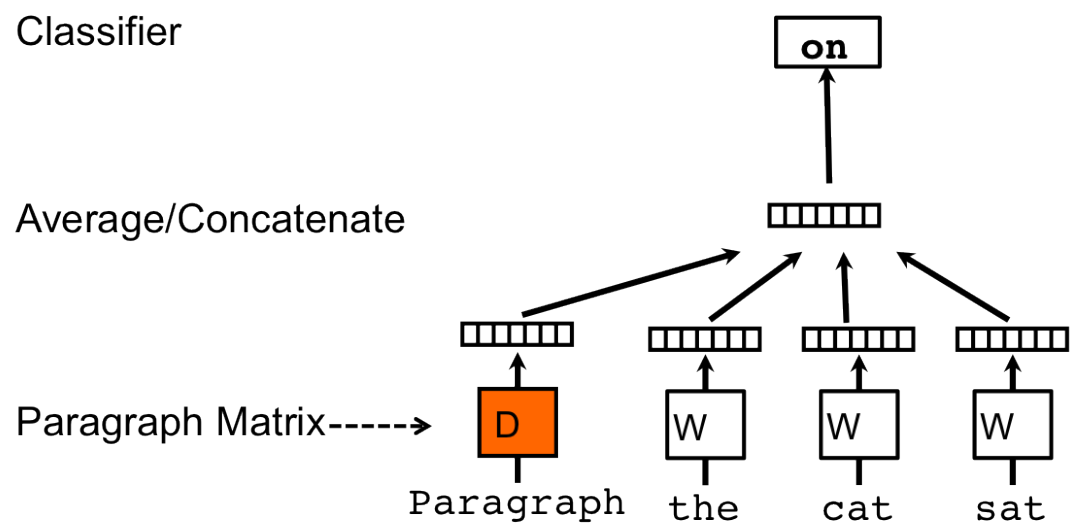
\includegraphics[scale=0.3]{figure/para-vec-1}
    \caption{Distributed Memory Model of Paragraph Vectors (PV-DM)\cite{ParagraphVec}}
    \label{fig:para-vec-1}
\end{figure}

\item Another way would be to just use the sentence presentation vector to guest which word it contains as in Fig.\ref{fig:para-vec-2}.

\begin{figure}[H]
    \centering    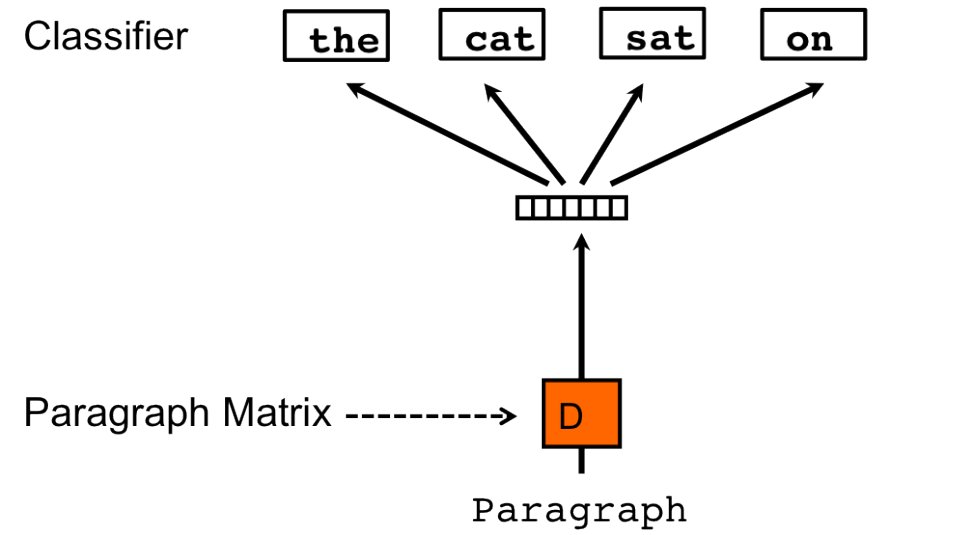
\includegraphics[scale=0.3]{figure/para-vec-2}
    \caption{Distributed Bag of Words version of Paragraph Vector (PV-DBOW)\cite{ParagraphVec}}
    \label{fig:para-vec-2}
\end{figure}

\item The third way was inspired by the recent successes of seq2seq learning\cite{SutskeverVL14}\cite{semisup-seq2seq}\footnote{A Pytorch implementation of seq2seq models can be found at \url{http://pytorch.org/tutorials/intermediate/seq2seq_translation_tutorial.html}}. 
This method use a RNN (e.g. Vanilla RNN, LSTM, GRU in Sec.\ref{sec:RNN}) to encode a sentence then use the same RNN to reconstruct it given its encoded vector\cite{semisup-seq2seq} as in Fig.\ref{fig:rnn-autoencoder}.
By unsupervised pre-train using this method on Amazon review (Sec.\ref{sec:amazon})), the authors were able to archive dramatic improvement on Rotten Tomatoes sentiment classification task. 

\begin{figure}[H]
    \centering    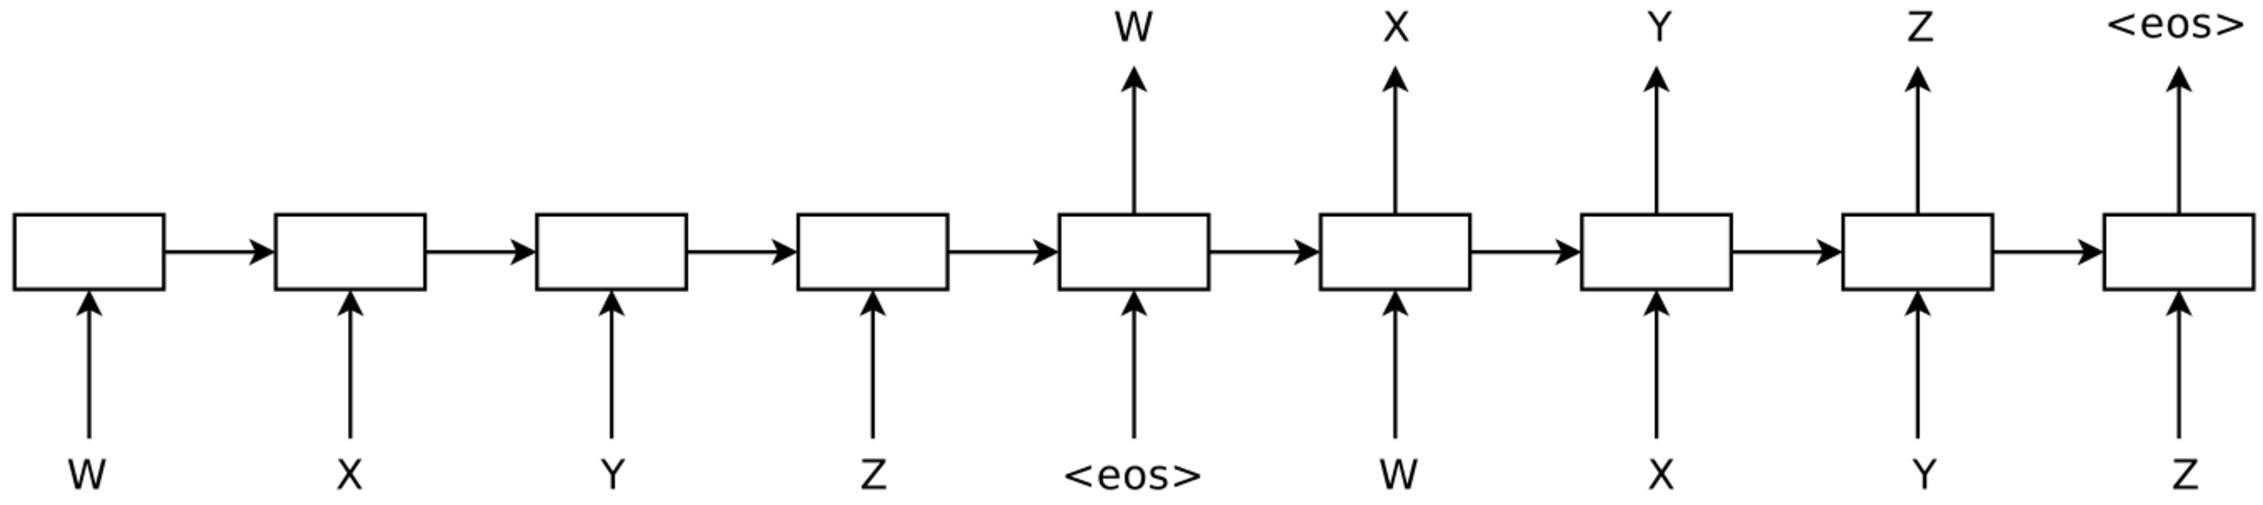
\includegraphics[scale=0.43]{figure/rnn-autoencoder}
    \caption{Sequence Autoencoder processing the sentence "WXYZ"\cite{semisup-seq2seq}.}
    \label{fig:rnn-autoencoder}
\end{figure}

\end{itemize}

\paragraph{An example of successfully applying unsupervised training technique to improve sentiment analysis on Stanford Sentiment Treebank}
One recent research\cite{2-layer-cnn} have demonstrated that applying unsupervised training can improve sentiment analysis task on Stanford Sentiment Treebank.

\begin{figure}
    \centering    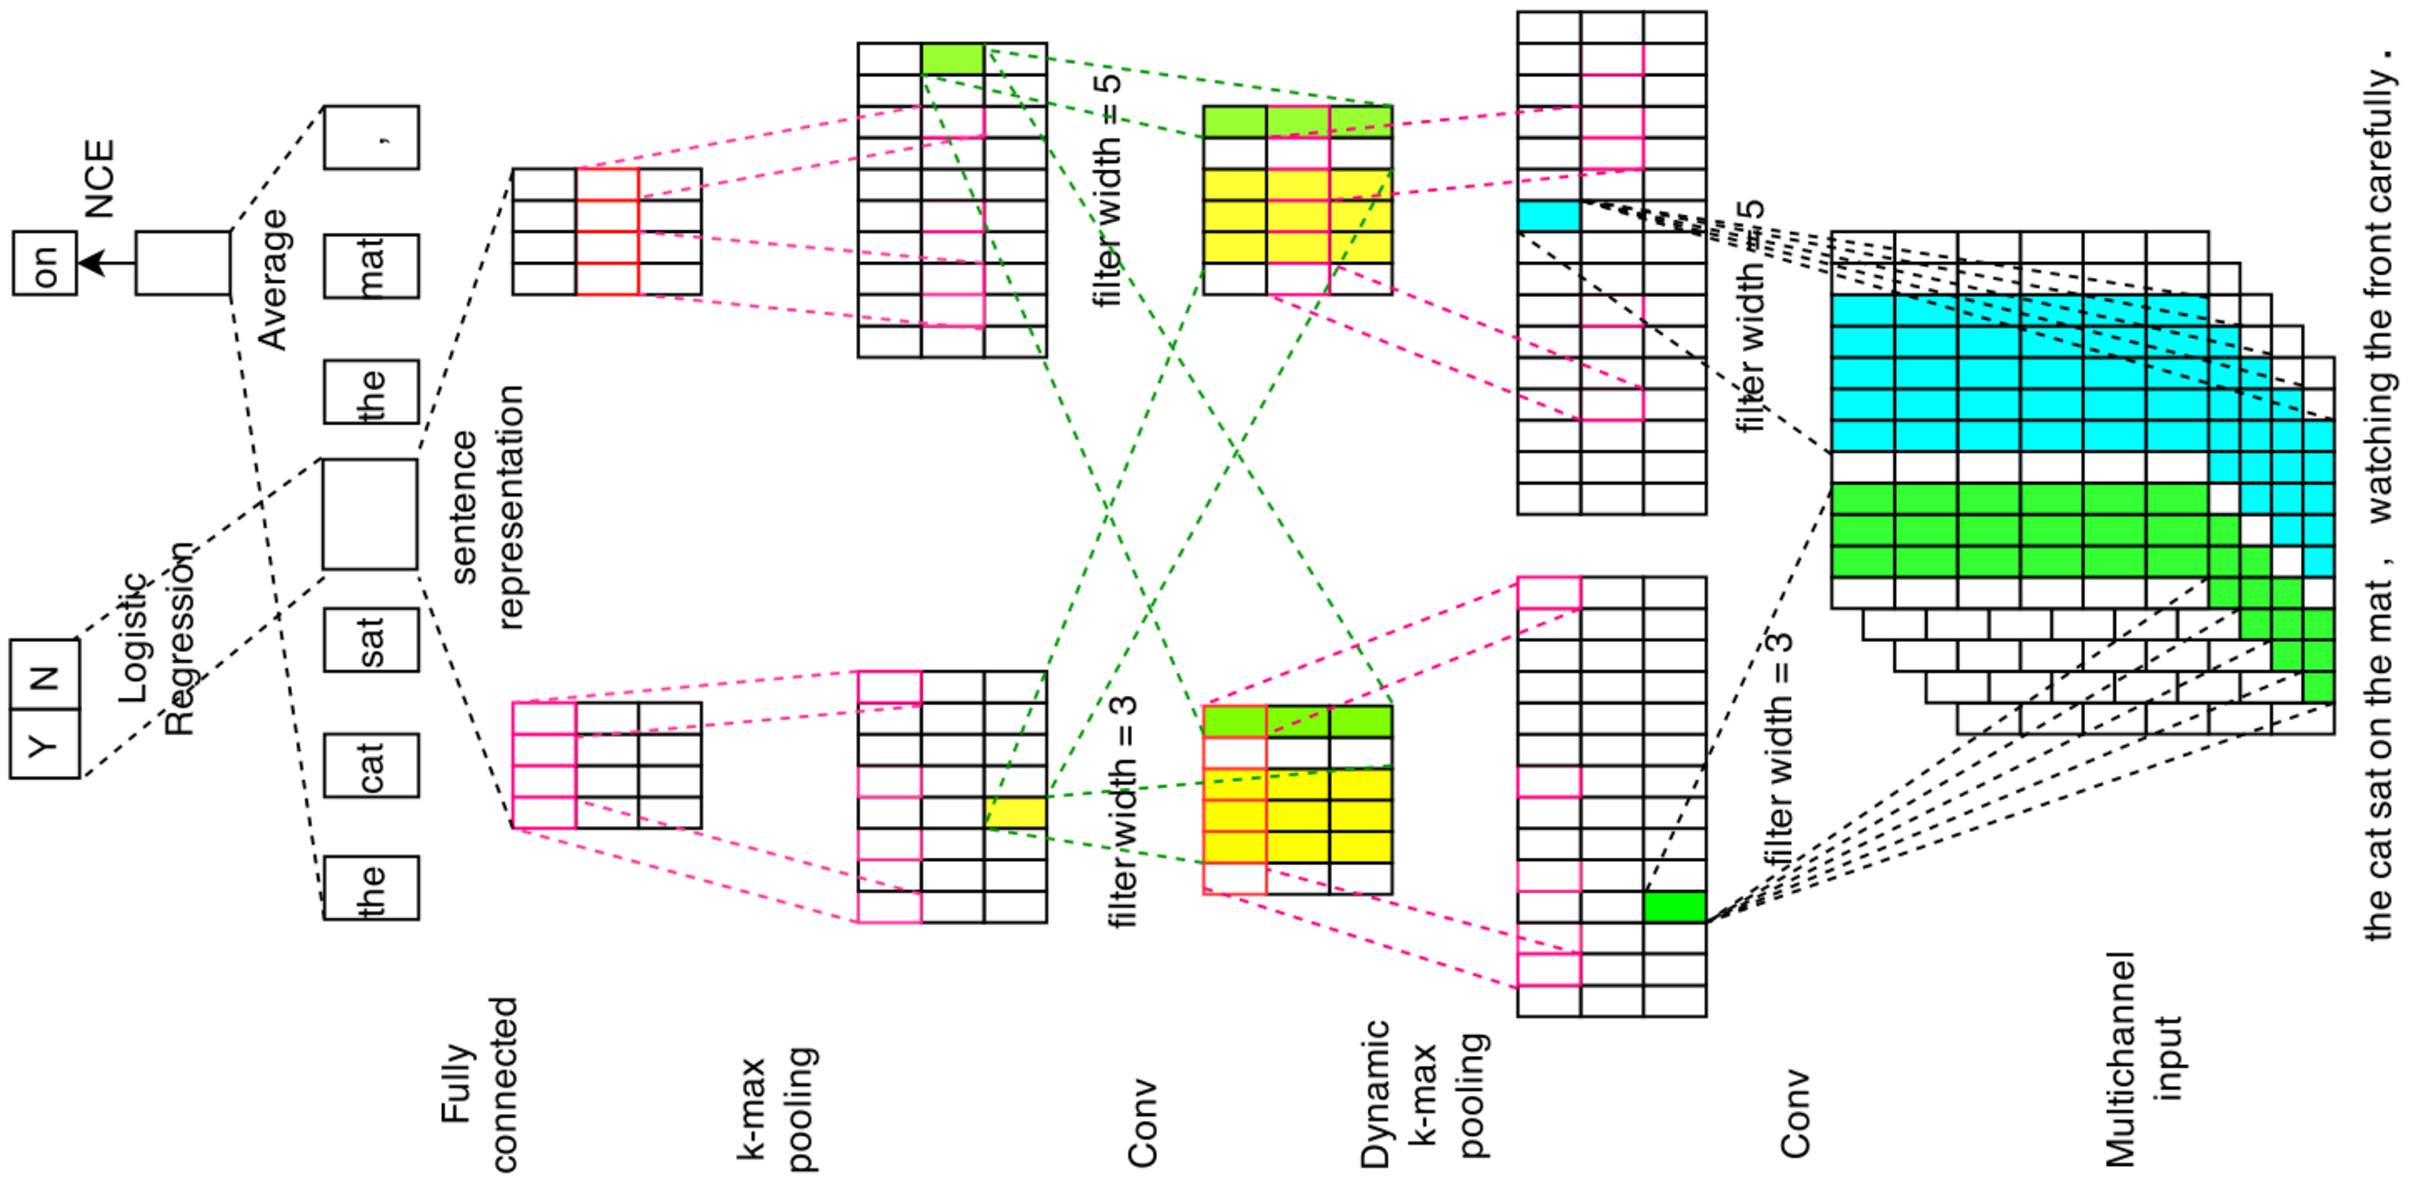
\includegraphics[scale=0.5, angle =-90 ]{figure/2-layer-cnn}
    \caption{Model architect of a multichannel 2-layer CNN during supervised and unsupervised training process\cite{2-layer-cnn}.}
    \label{fig:2-layer-cnn}
\end{figure}

As illustrated in Fig.\ref{fig:2-layer-cnn}, the first convolution layer and multichannel word embedding of this network similar to \hyperref[kim-cnn]{Yoon Kim's CNN architect}.
The difference appears after that, instead of using  \hyperref[sec:max-overtime-pooling]{max pooling overtime layer} to produce sentence encoding vector, the authors used Dynamic k-max Pooling\cite{deep-cnn-2014} layer with another convolution layer and a k-max pooling layer\cite{deep-cnn-2014}. 

With large number of parameter, their model prone to over-fitting, to tackle this problem, the authors unsupervised pre-train their model on large unlabeled data set using setting similar to Distributed Memory Model of Paragraph Vectors (PV-DM)\cite{ParagraphVec} (Fig.\ref{fig:para-vec-1}).
Given a model \(M\) which the authors want to pre-train, and a sentence \(s\) in the data set used for pre-training process, the sentence presentation \(p\) is computed as \(M(s)\). 
Define the context of the target word \(w_i\) as \(C = \{w_{i-t},\ldots,w_{i-1}, w_{i+1},\ldots,w_{i+t}\}\), the feature vector used to predict word \(w_i\) is computed by averaging word presentation vectors of the words in \(C\) and sentence encoding \(p\)\cite{2-layer-cnn}.
 
On overall, their system was able to archive accuracy of \(89.4\%\) on binary setting of sentiment analysis. 
With pre-training step removed from the training process, the model only archive accuracy of \(87.6\%\), which proved the significant contribution of pre-training step.\cite{2-layer-cnn}



\section{Distributed word presentation}\label{sec:distributed-word}

\subsection{Glove vectors}\label{sec:glove}
\subsubsection{Method}

\subsubsection{Results and Discussion}



\chapter{Method}
We evaluate our model on predict the sentiment of movies review. We use SST (See \ref{sec:sst}) to train and evaluate our model on binary classification task with given train/dev/test split 6920/872/1821 after remove neutral sentences. We preprocess the dataset according to our model.

\section{Improving sentence composition}

\subsection{Model VT Tree-GRU}\label{sec:VTtree}
\begin{figure}[H]
	\centering
	
\includegraphics[width=0.8\linewidth]{figure/vtgrusummary.pdf}
	\caption[Convolution Tree LSTM]{}
	\label{fig:vtgrusummary}
\end{figure}

\subsubsection{Embedding layer}
Embedding layer is a lookup table that convert input data (such as text) into its vector representation. A word embedding layer parameters is its embedding matrix $M  \in \mathbb{R}^{n \times d}$, where $n$ and $d$ is vocabulary size and embedding vector dimension, respectively. In practical, an embedding layer also come with vocabulary-index lookup table, which map word with index, which has vector representation corresponding to row in word embedding matrix.
  
The following step are require once for each experiment:
\begin{itemize}
	\item Build vocabulary-index lookup table
	\item Init/Load word embedding matrix corresponding to vocabulary-index table
	\item Convert every sentences in dataset into indices using vocabulary-index table  
\end{itemize}
Usually, indices are keep as dataset. Raw dataset (such as readable words) are discarded to free up memory. For each mini-batch, we use indices to lookup word representation vector from embedding matrix. Embedding matrix represent of each sentences in dataset are not saved and needed look-up every mini-batch for following reason.
\begin{itemize}
	\item Saved embedding matrix for each data sentences cost more memory than save only indices and look-up in embedding layer.
	\item Embedding matrix are trainable parameters and updated every iteration.
\end{itemize}

Figure \ref{fig:embeddinglayer} illustrates embedding layer component and describes the process of convert raw data sentence into its word representation.

\begin{figure}[H]
	\centering
	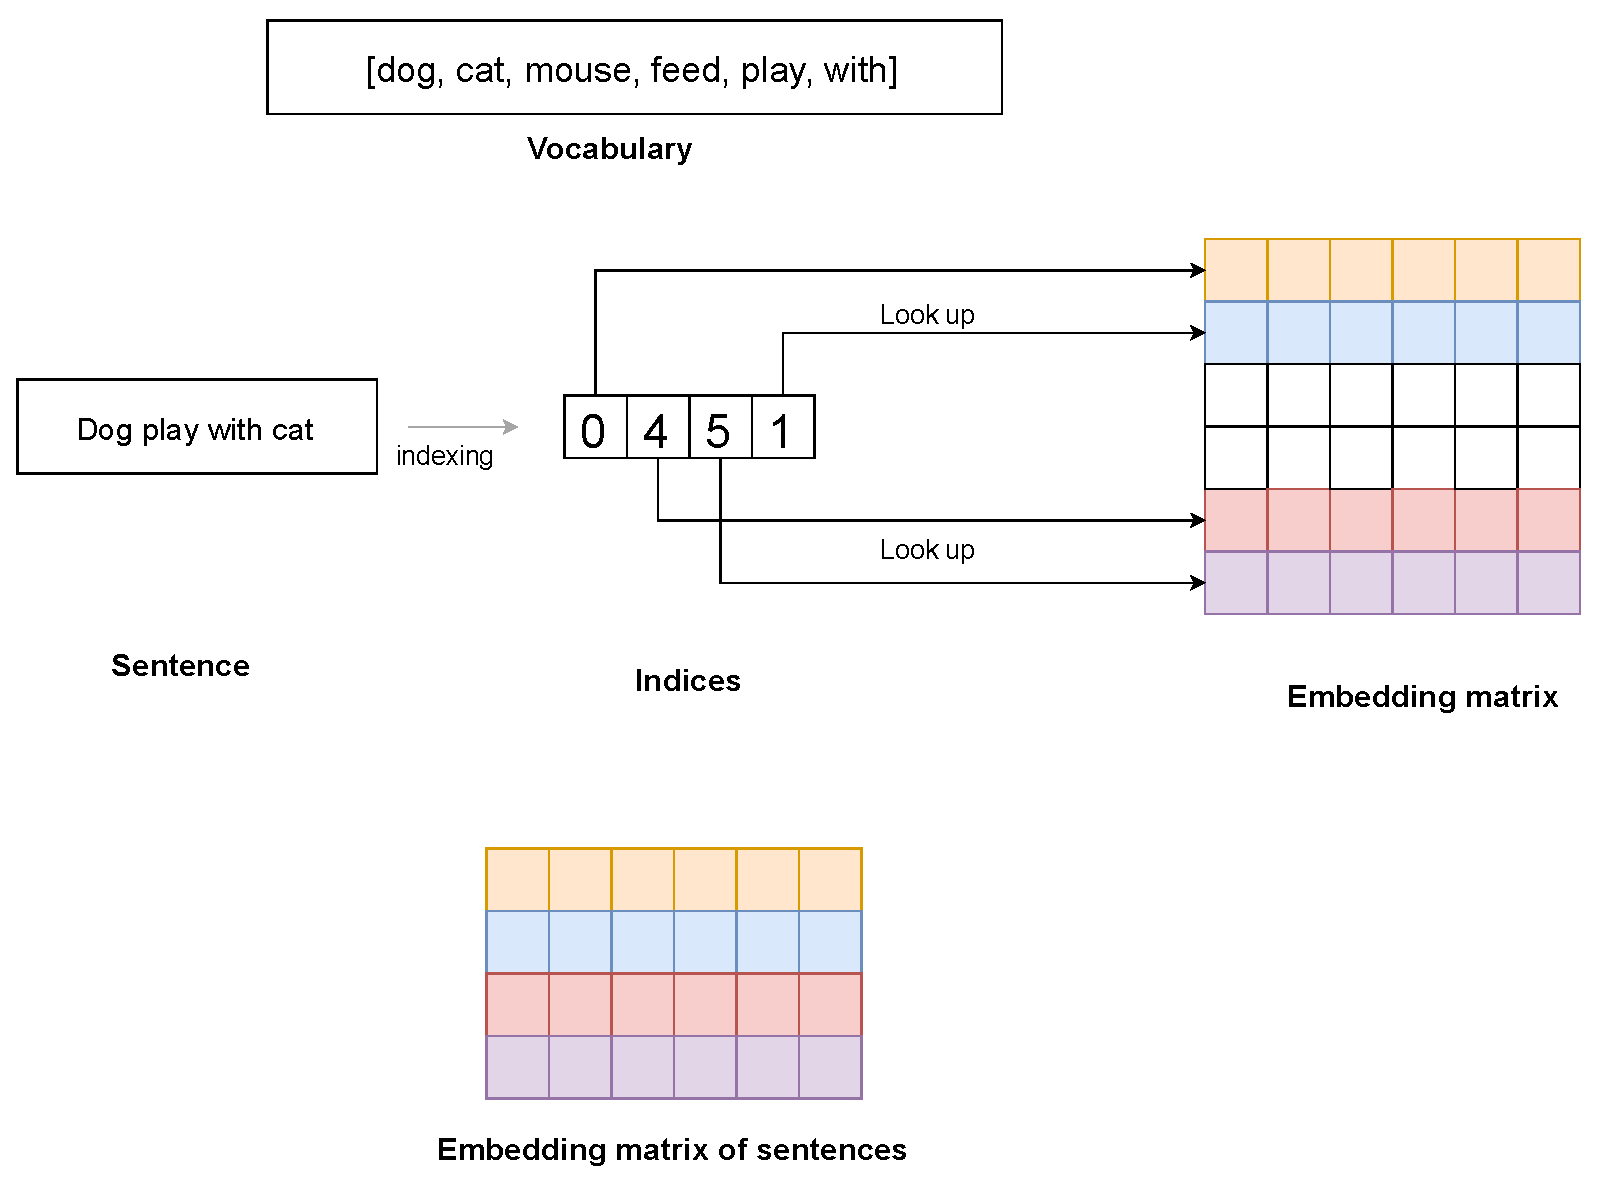
\includegraphics[width=0.9\linewidth]{figure/embeddinglayer.pdf}
	\caption[Overview of embedding layer]{Overview of Embedding Layer}
	\label{fig:embeddinglayer}
\end{figure}



\subsubsection{VT Tree-GRU}
We apply both tree structure network and recurrent structure in our model. In each sub-tree, which consist of one parent node with or without children, we apply recurrent network structure over current node and all its child. We store last hidden layer as node intermediate information and use as input to higher level. For network unit, we choose Gated Recurrent Unit (GRU), which was first introduced in \cite{cho2014learning}. GRU transition equation are describe in eq \ref{eq:gru}. 

\begin{equation}
\label{eq:gru}
\begin{aligned}
&r = sigmoid(W_{ir} x + b_{ir} + W_{hr} h + b_{hr}) \\
&i = sigmoid(W_{ii} x + b_{ii} + W_{hi} h + b_{hi}) \\
&n = \tanh(W_{in} x + b_{in} + r * (W_{hn} h + b_{hn})) \\
&h' = (1 - i) * n + i * h\\
\end{aligned}
\end{equation}

\subsubsection{Constituency VT Tree-GRU} \label{sec:VTtreeConstituency}
SST (See \ref{sec:sst}) given format is binary constituency parse tree. We use CoreNLP \cite{manning2014stanford} to create non-binary constituency parse tree and annoted Part-of-speech tag (POS-tag) for each node. We use word and tag and tree structure as input for our model.

For each sub-tree, we sort child node from left to right order. We take node state k, node POS-tag, and parent POS-tag as input for GRU timestep. We put parent node at the end of GRU chain. We take hidden state of last timestep as node state k for parent node. For a sub tree fig \ref{fig:treecp}, model is illustrate in \ref{fig:cvtgru}. For leaf node case, we input word and tag into GRU and get hidden output h as k for leaf node as fig \ref{fig:gruleaf}.
\begin{figure}[H]
	\centering
	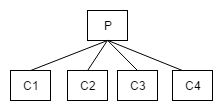
\includegraphics[width=0.5\linewidth]{figure/treecp}
	\caption[A sub tree with parent and children node]{A sub tree with parent and children node}
	\label{fig:treecp}
\end{figure}

\begin{figure}[H]
	\centering
	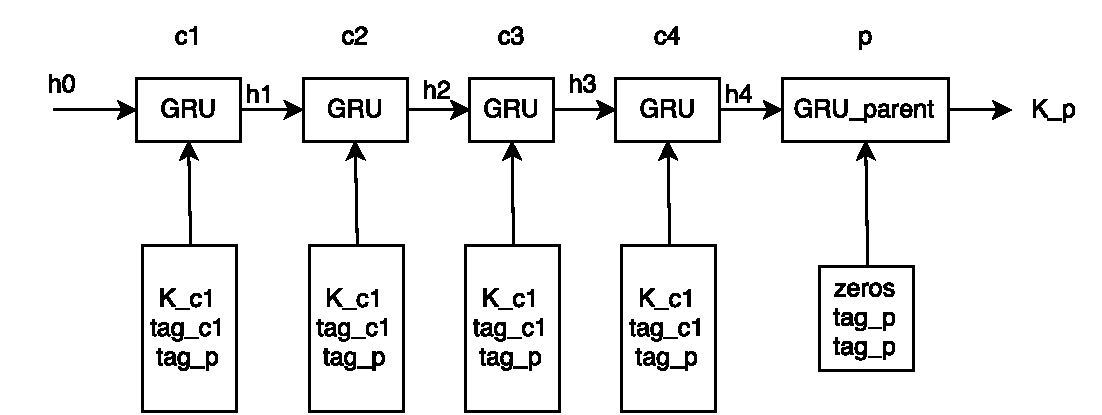
\includegraphics[width=0.7\linewidth]{figure/cvtgru}
	\caption[Constituency VT Tree-GRU]{Constituency VT Tree-GRU}
	\label{fig:cvtgru}
\end{figure}

\begin{figure}[H]
	\centering
	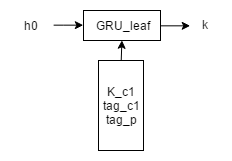
\includegraphics[width=0.4\linewidth]{figure/gruleaf}
	\caption[Constituency VT Tree-GRU leaf case]{Constituency VT Tree-GRU leaf case}
	\label{fig:gruleaf}
\end{figure}



\subsubsection{Dependency VT Tree-GRU} \label{sec:VTtreeDependency}
We use \cite{manning2014stanford} to create dependency parse tree with annoted POS-tag and labeled Universal Dependencies between head word and its dependents.

We build a model similar to constituency case, with a chain GRU for each sub tree. However, we does not put parent node at the end of the chain. Instead, parent node and child node are sorted according to their position in sentences. We take node state k, node POS-tag, node dependency relationship type vs head word as input for GRU timestep. At parent node, we set dependency relationship type is 'self' and node states k set to zeros vector. We take hidden state of last timestep as node state k for parent node. In case of leaf node, we treat it as parent node without children. We build GRU chain with only parent node for leaf case. Fig \ref{fig:dependencyvtgru} illustrate Dependency VT GRU model.

\begin{figure}[h]
	\centering
	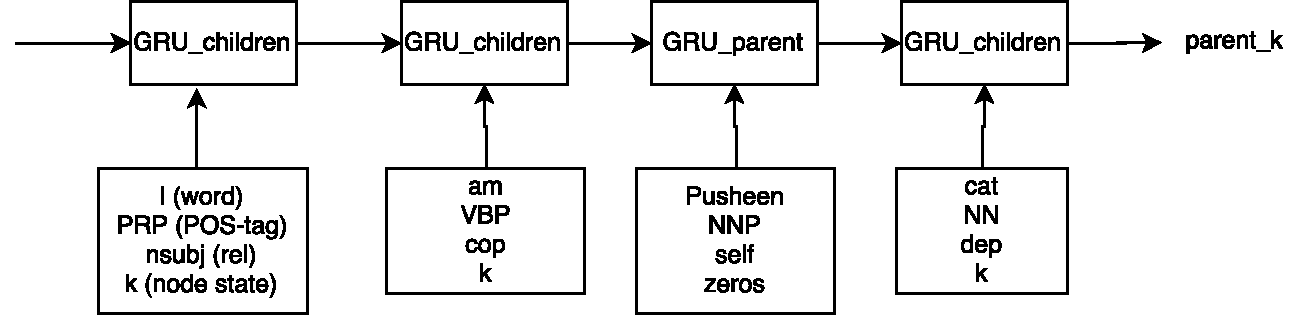
\includegraphics[width=0.5\linewidth]{figure/dependencyvtgru}
	\caption[Dependency VT GRU]{Dependency VT GRU}
	\label{fig:dependencyvtgru}
\end{figure}

\subsubsection{Output layer and loss function}
We use softmax classifier and cross entropy loss function as described in \cite{treeLSTM}.  For each parent labeled node, we use node state $k$ as input to output layer and calculate loss against given label. Root node state $k$ is used to determine sentiment of whole sentences.

\subsubsection{Training method and hyper-parameter}
We preprocess SST as described in \ref{sec:VTtreeConstituency} and \ref{sec:VTtreeDependency}. We use default train/dev/test split after remove neutral sentences (6920/872/1821). We only remove neutral sentence, but keep neutral text span of positive or negative sentences. 

We init our word representation with pretrained word vector (Glove \cite{glove}, paragram\_xxl \cite{wieting2015towards}) with default dimension of 300.  We initialize randomly tag and relationship representation (dependency only) vector of dimension 50. We set memory dimensions of 150.

Our model was trained using AdaGrad \cite{duchi2011adaptive} with learning rate of 0.05, L2 regularization of 0.0001, batch size of 25. We manually update our word representation with learning rate $\alpha$ of 0.05 as equation \ref{eq:manuallyupdate}. 

\begin{equation}
\label{eq:manuallyupdate}
w = w - \alpha\delta J(\theta)
\end{equation}


\subsection{CNN-TreeLSTM}\label{sec:CNNtree}
\begin{figure}[H]
	\centering
	
\includegraphics[width=0.8\linewidth]{figure/convtreelstmsummary}
	\caption[Convolution Tree-LSTM overview]{Convolution Tree-LSTM overview}
	\label{fig:convtreelstmsummary}
\end{figure}
CNN-TreeLSTM is a combination of Convolution Neural Network with Tree-LSTM \cite{socher2013recursive}.

\subsubsection{Convolution layer}
Each convolution layer contain n filter. Each filter has dimension $w x d$, with d is word vector dimensions and w is word-level kernel size. We may have one or more kernel size, with are treat as model hyper-parameter. 

We align the first axis of each feature map with the embedding axis and convolve along first dimension of embedding matrix. We use 'half' convolutions which each filter produce a 1d vector have same length as sentence length. Thus, n filter produces $l x n$ matrix with $l$ is sentence length. We set $n = d$ in order to produce output with same dimension as embedding matrix. 

\begin{figure}[H]
	\centering
	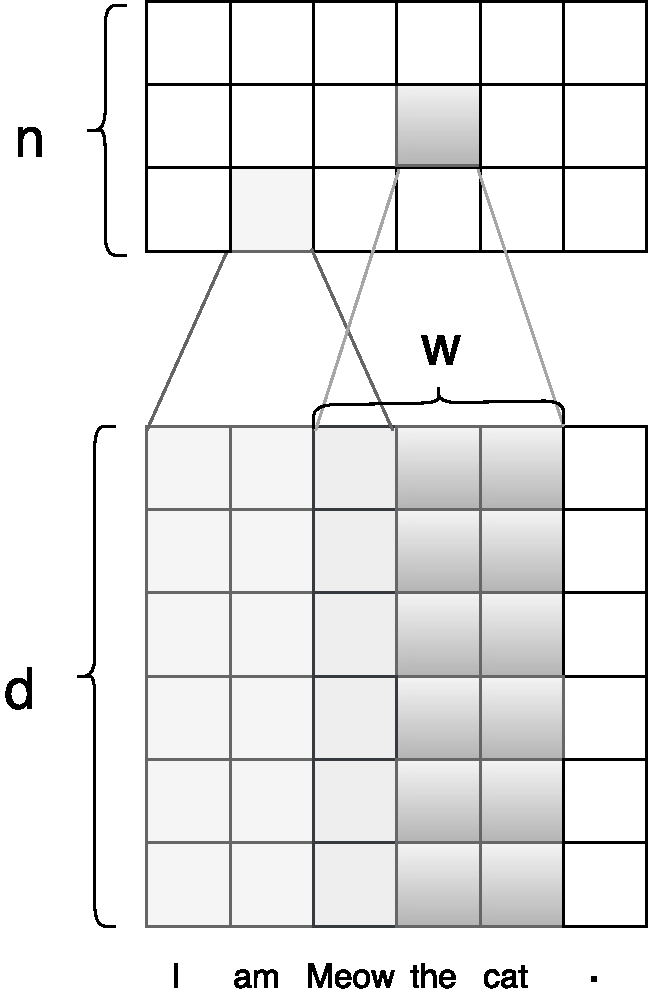
\includegraphics[width=0.6\linewidth]{figure/convlayer}
	\caption[Convolution layer]{Convolution layer}
	\label{fig:convlayer}
\end{figure}

\subsubsection{Training method and hyper-parameter}





\section{Improving continuous distributed word presentation}

\subsection{Training Glove embedding on Amazon reviews data set}

\subsection{Using hierarchical CNN to improve Glove embedding}

\subsubsection{Training method and hyper-parameter}


\section{Combining better sentence composition and distributed word presentation}

\subsubsection{Training method and hyper-parameter}


\hypertarget{chap:result}{\chapter{Results and Discussion}}\label{result-discuss}


\section{Improving sentence composition}
Experiment results are summaries in Table \ref{table:experimentresult}. In all of our model, we updated word vector manually (eq. \ref{eq:updated}) yield better result than using Adam, Adagrad or Adadelta. 

\begin{table}[H]
	\centering
	\caption{Experiment result. For our experiment, we report mean accuracies of 5 runs. Max value in bracket.}
	\label{table:experimentresult}
	\begin{tabular}{ll}
		Method                                   & Binary \\ \hline
		LSTM                                     & 86.40   \\
		BiLSTM                                   & 85.80   \\ \hline
		Constituency Tree-LSTM \cite{treeLSTM} & 88.00     \\
		Constituency Tree-LSTM \cite{treeLSTM} (Glove Amazon) & 88.85 (89.35) \\
		Dependency Tree-LSTM  \cite{treeLSTM}  & 85.70   \\ 
		CNN GRU \cite{cnn-rnn}					& 89.13(89.95) *	\\
		CNN LSTM \cite{cnn-rnn}					& 89.43(89.56) *	\\ \hline
		Constituency VT Tree-GRU                 & 87.65 (88.25)  \\
		Dependency VT Tree-GRU                   & 87.13  (88)  \\ \hline
		CNN LSTM 								& 89.10 (89.40)      \\
		% CNN LSTM (pretrained)** 				&			\\ 
		2 Channel CNN LSTM						& 89.54	(89.79)	\\
		% 2 Channel CNN LSTM (pretrained)**		& 		\\
		CNN Tree-LSTM                            & 88.82 (88.92) \\
		CNN Tree-LSTM (Glove Amazon) 			& 88.96 (89.18) \\
		2 Channel CNN Tree-LSTM  				& 89.66 (90.12)
	\end{tabular}
\end{table}

\textit{(*): average of 5 runs on their implementation \footnote{https://github.com/ultimate010/crnn}} and result claim in their paper (in bracket).

% \textit{(***): CNN and LSTM layer are initialize using pre-trained parameters from Section \ref{sec:CNNtree}}

\subsection{VT Tree-GRU}
Our dependency VT Tree-GRU outperformed Dependency Tree-LSTM on same dependency dataset. Constituency VT Tree-GRU model slightly better than Dependency VT Tree-GRU. This performance gap is expected due to dependency parse tree has less labeled node comparing to constituency parse tree, which has been explained in \cite{treeLSTM}. We discovered that train model composition with Adam learning rate of 0.001 and word representation (updated manually) learning rate at 0.05 for 20 epochs yield best result. Training more epochs does not improve the performing.


\subsection{CNN Tree-LSTM and 2 channel CNN Tree-LSTM}
We found that 100 filters of size 3 words and 100 filters of size 5 words yield better result comparing to single filters size or number of filters larger than 200. We trained with Adagrad of learning rate of 0.01 and word vectors (updated manually) at learning rate 0.1 give best result. We trained for 60 epochs

Two input channel CNN Tree-LSTM has better accuracy than one input channel CNN Tree-LSTM because additional data are incorporated in a second word embedding matrix, which is trained on Amazon Review Dataset.

%\subsection{Model VT Tree-GRU}


%\subsubsection{Constituency}

%\subsubsection{Dependency}


\section{Improving continuous distributed word presentation}

\subsection{Training Glove embedding on Amazon reviews data set}

\subsection{Using hierarchical CNN to improve Glove embedding}


\section{Combining better sentence composition and distributed word presentation}


\hypertarget{chap:conclude}{\chapter{Conclusion}}\label{conclusion}
\section{Contributions of this thesis}
In search of new improvements on the task of sentence-level sentiment analysis, we have tried three approaches: Utilizing local syntactic information at each node of Recursive Neural Networks; Transfer Learning by retraining Glove on Amazon Reviews dataset and Combining Recursive Neural Networks with Convolution Neural Networks.
Based on our results in Table.\ref{table:experimentresult}, \textbf{hypotheses that supported by our results including}:
\begin{itemize}
\item Amazon Glove captured some good\footnote{good for the task of sentiment analysis of movie reviews} features that dose not exist or hardly be extracted in Glove Common Crawl. (Sec.\ref{proved:Amazon-adv-Common})

\item There are some good features dose not appear in Glove Amazon but only appear in Glove Common Crawl or when combining both Glove Amazon and Glove Common Crawl. (Sec.\ref{proved:Common-syn-Amazon})

\item By adding a convolution layer before the leaf-node of Tree-LSTM, convolution layer will help Tree-LSTMss to mitigate the problem of lacking local context and weak feature capturing at leaf nodes (Sec.\ref{sec:tree-discuss}).
Mutually, using Tree-LSTM to combine the feature maps produced by convolution layer is better than max-over-time pooling layer (Sec.\ref{kim-drawback}). (Sec.\ref{proved:tree-conv-benefit})

\item  Tree-LSTMs have already utilized the information in word embeddings and the local syntactic information from tag embeddings adding no more value. (Sec.\ref{unproved:tag-useless})
\end{itemize}
\bigbreak
\label{unproved-hypo}
\textbf{Hypotheses that we have not had efficient data to support or oppose}:
\begin{itemize}
\item Unsupervised pre-training methods (on Amazon Reviews) can help improving Multichannel CNN LSTM and Multichannel CNN Tree-LSTM. (Sec.\ref{sec:unsupervised-pretrain})

\item  Unsupervised pre-training Multichannel CNN LSTM as Language Model on Amazon Reviews can help it to learn knowledge about Film industry or human culture in forms of: features in word embeddings; parameters in convolution filters and LSTM unit. (Sec.\ref{lm-hypothesis})

\item CNN Tree-LSTM performed worst than CNN LSTM, the reason might be because of over-fitting. (Sec.\ref{unproved:cnn-treelstm-overfit})
\end{itemize}

\section{Future works}
We will do experiments to have efficient data to support or oppose the unproved hypotheses above.
We will also re-evaluate our models and methods on Stanford Sentiment Treebank with fine-grained setting.

% Công trình của tác giả (nếu không có thì comment 02 dòng dưới)
\addcontentsline{toc}{chapter}{Danh mục công trình của tác giả}
\chapter*{Danh mục công trình của tác giả}
\label{Appendix1}

\begin{enumerate}
\item Tạp chí ABC
\item Tạp chí XYZ
\end{enumerate}

% In tài liệu tham khảo
\addcontentsline{toc}{chapter}{TABLE OF CONTENTS}
\printbibheading[title={TABLE OF CONTENTS}]

% \printbibliography[heading=subbibliography, title={Vietnamese}, keyword=Viet, resetnumbers=true]

\DeclareNameAlias{sortname}{last-first}
\DeclareNameAlias{default}{last-first}

\printbibliography[heading=subbibliography, title={English}, notkeyword=Viet, resetnumbers=4] 
% ===================================================================== %
% CHÚ Ý: phải gán lại resetnumbers=số tài liệu tham khảo tiếng Việt + 1 %
% ===================================================================== %

% Phần phụ lục
\appendix

\chapter{APPENDICES 1}
\label{Appendix1}

\begin{figure} [H]
	\begin{minipage}{\textwidth}
		\centering
		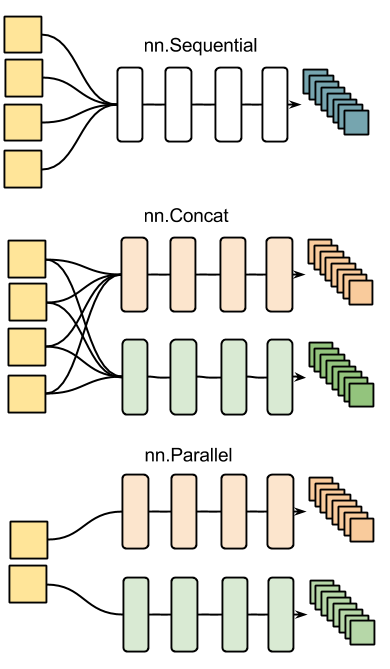
\includegraphics[width=0.5\linewidth]{figure/nncontainer}
		\caption[Torch nn container]{Torch nn container \footnote{ \url{https://github.com/soumith/cvpr2015/blob/master/Deep\%20Learning\%20with\%20Torch.ipynb}}}
		\label{fig:nncontainer}
	\end{minipage}
\end{figure}

\begin{lstlisting}[caption={MLP using nngraph},label={lst:torchtrain}, language={[5.1]Lua}]
require 'nn'
require 'optim'

model = nn.Sequential()
model:add(nn.Linear(1,1))

criterion = nn.MSECriterion()

x = torch.Tensor{{1,2,3,4,5,6,7,8,9,10}}
x = x:t()
y = torch.Tensor{{3,5,7,9,11,13,15,17,19,21}}
y = y:t()

params, gradParams = model:getParameters()

function feval(params)
gradParams:zero()
local outputs = model:forward(x)
local loss = criterion:forward(outputs,y)
local dloss_doutput = criterion:backward(outputs,y)
model:backward(x, dloss_doutput)
return loss, gradParams
end

local optimState = {
learningRate = 0.01
}

for epoch = 1, 100 do
optim.sgd(feval,params, optimState)
end

test = torch.Tensor{{1,3,5,7,9,11,100}}
test = test:t()

print (model:forward(test))
\end{lstlisting}



\begin{lstlisting}[caption={Theano MLP},label={lst:theanomlp}, language={python}]
import numpy as np
import theano
import theano.tensor as T
import theano.tensor.nnet as nnet

class MLP:
def __init__(self):
x = T.dvector()
y = T.dscalar()
t1 = np.array(np.random.rand(3, 3), dtype=theano.config.floatX)
theta1 = theano.shared(t1)  # 3x3 weight matrix
t2 = np.array(np.random.rand(4, 1), dtype=theano.config.floatX)
hid1 = MLP.sigmoid_layer(x, theta1)  # hidden layer
theta2 = theano.shared(t2)  # 4x1 weight matrix
output_layer = T.sum(MLP.sigmoid_layer(hid1, theta2))
fc = (output_layer - y)**2
self.cost = theano.function(inputs=[x,y], outputs = fc,updates=[
(theta1, Xor.grad_desc(fc, theta1)),
(theta2, Xor.grad_desc(fc, theta2))
])
self.run_forward = theano.function(inputs=[x],outputs=output_layer)

@staticmethod
def sigmoid_layer(x, w):
b = np.array([1], dtype=theano.config.floatX)
new_x = T.concatenate([x,b])
m = T.dot(w.T, new_x)
h = nnet.sigmoid(m)
return h


@staticmethod
def grad_desc(cost, theta):
alpha = 0.1
return theta - (alpha* T.grad(cost, wrt=theta))

def forward(self, x):
output = self.run_forward(x)
return output


def train(self, train_x, train_y, n_epoch):
cur_cost = 0
for epoch in range(n_epoch):
for i in range(len(train_x)):
cur_cost = self.cost(train_x[i],train_y[i])
if epoch % 1000 == 0:
print(cur_cost)
print ('train complete')
\end{lstlisting}

\chapter{APPENDICES 2}
\label{Appendix2}

Đây là phụ lục 2.



\end{document} 